%!TEX output_directory = target
% Currently this document is written in German
% !TeX spellcheck = de_DE

%Ensure that all odl school LaTeX habits are remarked
\RequirePackage[l2tabu, orthodox]{nag}
%Neue deutsche Trennmuster
%Siehe http://www.ctan.org/pkg/dehyph-exptl und http://projekte.dante.de/Trennmuster/WebHome
%Nur für pdflatex, nicht für lualatex
\RequirePackage[ngerman=ngerman-x-latest]{hyphsubst}
% \documentclass{lni}
% in Englisch stattdessen:
\documentclass[english]{lni}







%% Some packages, no need to be adabted

% enable copy and paste of ligatures (e.g., in "workflow" and umlauts)
\usepackage{cmap}

%Überschrift des Literaturverzeichnisses
%Only in German
\iflnienglish
\else
\renewcommand{\refname}{Literaturverzeichnis}
\fi

%Enable input of umlauts using UTF-8.
\usepackage[utf8]{inputenc}

\usepackage{graphicx}

\usepackage{fancyhdr}

%Kopf- und Fußzeileneinstellungen
\fancypagestyle{lnifirstpage}{
% Löscht alle Kopf- und Fußzeileneinstellungen
\fancyhf{}

%Kopfzeile
\fancyhead[RO]{\small Einreichung für: <Konferenz/Workshop>,\linebreak%
Geplant als Veröffentlichung innerhalb der Lecture Notes in Informatics (LNI)
}
%Für den Herausgeber:
%\fancyhead[RO]{\small <Vorname Nachname [et.\ al.\ ]>(Hrsg.): <Buchtitel>,\linebreak%
%Lecture Notes in Informatics (LNI), Gesellschaft für Informatik, Bonn <Jahr> \hspace{5pt} \thepage \hspace{0.05cm}}

%Linie unter Kopfzeile
\renewcommand{\headrulewidth}{0.4pt}
}

% Put in the short title (Kurztitle) here
\fancypagestyle{lni}{
\fancyhf{}
%Zu lange Titel müssen von den HerausgeberInnen gekürzt werden, Vorschläge der AutorInnen dazu sind herzlich willkommen.
\fancyhead[RO]{\small Gilbert: Declarative Sparse Linear Algebra on Massively Parallel Dataflow Systems \hspace{5pt}
\thepage \hspace{0.05cm}}
\fancyhead[LE]{\hspace{0.05cm}\small \thepage \hspace{5pt}
%Bis zu drei AutorInnen werden alle angeführt, darüber hinaus wird nur die erste Autorin bzw. der erste Autor angeführt und alle Weiteren mit et al.\ abgekürzt.
%Zu lange AutorInnenlisten müssen von den HerausgeberInnen gekürzt werden.
Till Rohrmann, Sebastian Schelter, Tilmann Rabl and Volker Markl}
\renewcommand{\headrulewidth}{0.4pt}
}

%if lstlistings is used
%better approach: use the minted package - see https://en.wikibooks.org/wiki/LaTeX/Source_Code_Listings#The_minted_package
\usepackage{listings}

\iflnienglish
\usepackage[figurename=Fig., tablename=Tab., font=small]{caption}
\else
\usepackage[figurename=Abb., tablename=Tab., font=small]{caption}
\fi

% Listingname heißt nun List.
\renewcommand{\lstlistingname}{List.}

\usepackage[T1]{fontenc}


%for demonstration purposes only
\usepackage[math]{blindtext}

%tweak \url{...}
\usepackage{url}
\urlstyle{same}
%improve wrapping of URLs - hint by http://tex.stackexchange.com/a/10419/9075
\makeatletter
\g@addto@macro{\UrlBreaks}{\UrlOrds}
\makeatother

%diagonal lines in a table - http://tex.stackexchange.com/questions/17745/diagonal-lines-in-table-cell
%slashbox is not available in texlive (due to licensing) and also gives bad results. Thus, we use diagbox
%\usepackage{diagbox}

\usepackage{booktabs}

%required for pdfcomment later
\usepackage{xcolor}

%for easy quotations: \enquote{text}
%also required by biblatex
\usepackage{csquotes}
\usepackage[
  backend=biber,
  style=LNI
]{biblatex}

% new packages BEFORE hyperref
% See also http://tex.stackexchange.com/questions/1863/which-packages-should-be-loaded-after-hyperref-instead-of-before

%enable hyperref without colors and without bookmarks
\usepackage[
%pdfauthor={},
%pdfsubject={},
%pdftitle={},
%pdfkeywords={},
bookmarks=false,
breaklinks=true,
colorlinks=true,
linkcolor=black,
citecolor=black,
urlcolor=black,
pdfpagelayout=SinglePage,
pdfstartview=Fit
]{hyperref}
%enables correct jumping to figures when referencing
\usepackage[all]{hypcap}

%enable nice comments
\usepackage{pdfcomment}
\newcommand{\commentontext}[2]{\colorbox{yellow!60}{#1}\pdfcomment[color={0.234 0.867 0.211},hoffset=-6pt,voffset=10pt,opacity=0.5]{#2}}
\newcommand{\commentatside}[1]{\pdfcomment[color={0.045 0.278 0.643},icon=Note]{#1}}

%compatibality with TODO package
\newcommand{\todo}[1]{\commentatside{#1}}

% we have to load the user defined packages here in order to not mess up with cleveref
%!TEX root=paper.tex
\usepackage{tikz}

\usepackage{amssymb}
\usepackage{amsmath}

\usepackage{newfloat}
\DeclareFloatingEnvironment[
  fileext=lol,
  name=Listing
]{listing}

\usepackage[labelformat=simple]{subcaption}

\DeclareCaptionSubType{listing}
\renewcommand\thesublisting{(\alph{sublisting})}

\newcommand{\code}[1]{\texttt{#1}}

\newlength\dualpgfwidth
\setlength\dualpgfwidth{.5\linewidth}

\usepackage{pgfplots}
\pgfplotsset{compat=1.14}

%enable \cref{...} and \Cref{...} instead of \ref: Type of reference included in the link
\iflnienglish
\usepackage[capitalise,nameinlink]{cleveref}
%Nice formats for \cref
\crefname{section}{Sect.}{Sect.}
\Crefname{section}{Section}{Sections}
\crefname{figure}{Fig.}{Fig.}
\Crefname{figure}{Figure}{Figures}
\else
\usepackage[ngerman,capitalise,nameinlink]{cleveref}
\fi

%introduce \powerset - hint by http://matheplanet.com/matheplanet/nuke/html/viewtopic.php?topic=136492&post_id=997377
\DeclareFontFamily{U}{MnSymbolC}{}
\DeclareSymbolFont{MnSyC}{U}{MnSymbolC}{m}{n}
\DeclareFontShape{U}{MnSymbolC}{m}{n}{
    <-6>  MnSymbolC5
   <6-7>  MnSymbolC6
   <7-8>  MnSymbolC7
   <8-9>  MnSymbolC8
   <9-10> MnSymbolC9
  <10-12> MnSymbolC10
  <12->   MnSymbolC12%
}{}
\DeclareMathSymbol{\powerset}{\mathord}{MnSyC}{180}

%improve float placement
%source: http://people.cs.uu.nl/piet/floats/node1.html
%see also: http://tex.stackexchange.com/a/35130/9075
\renewcommand{\textfraction}{0.05}
\renewcommand{\topfraction}{0.95}
\renewcommand{\bottomfraction}{0.95}
\renewcommand{\floatpagefraction}{0.35}
\setcounter{totalnumber}{5}

%enable margin kerning
\usepackage{microtype}

% correct bad hyphenation here
\hyphenation{net-works semi-conduc-tor}

%%% Adapt to your needs from here

%Beginn der Seitenzählung für diesen Beitrag
\setcounter{page}{1}

\author{
Till Rohrmann\footnote{Apache Software Foundation, trohrmann@apache.org} \, %
Sebastian Schelter\footnote{Technische Universität Berlin, sebastian.schelter@tu-berlin.de} \, %
Tilmann Rabl\footnote{Technische Universität Berlin / DFKI, rabl@tu-berlin.de} \, %
Volker Markl\footnote{Technische Universität Berlin / DFKI, volker.markl@tu-berlin.de} \, %
}

\title{Gilbert: Declarative Sparse Linear Algebra\\ on Massively Parallel Dataflow Systems}

\bibliography{paper}

\begin{document}
\maketitle

%hint by http://tex.stackexchange.com/a/30229/9075 and http://tex.stackexchange.com/a/247652/9075
\thispagestyle{lnifirstpage}
\pagestyle{lni}

%Auf Anzahl der AutorInnen setzen, damit die weitere Nummerierung der Fußnoten passt
%Dieser Befehl \verb|\setcounter{footnote}{2}| legt in dem Fall fest, dass 2 Fußnotennummern bereits für die AutorInnen verbraucht wurden, damit die darauf folgenden Fußnoten mit der richtigen Nummerierung (ab 3) fortfahren. Dieser Wert muss an die jeweilige Zahl an AutorInnen bzw. bereits verbrauchte Fußnoten angepasst werden, sofern im weiteren Verlauf Fußnoten verwendet werden.
\setcounter{footnote}{2}

\begin{abstract}
In recent years, the generated and collected data is increasing at an almost exponential rate. 
At the same time, the data's value has been identified in terms of insights that can be provided. 
However, retrieving the value requires powerful analysis tools, since valuable insights are buried deep in large amounts of noise. 
Unfortunately, analytic capacities did not scale well with the growing data. 
Many existing tools run only on a single computer and are limited in terms of data size by its memory. 
A very promising solution to deal with large-scale data is scaling systems and exploiting parallelism.

In this paper, we propose Gilbert, a distributed sparse linear algebra system, to decrease the imminent lack of analytic capacities. 
Gilbert offers a MATLAB\textsuperscript{\textregistered}-like programming language for linear algebra programs, which are automatically executed in parallel. 
Transparent parallelization is achieved by compiling the linear algebra operations first into an intermediate representation. 
This language-independent form enables high-level algebraic optimizations.
Different optimization strategies are evaluated and the best one is chosen by a cost-based optimizer. 
The optimized result is then transformed into a suitable format for parallel execution. 
Gilbert generates execution plans for Apache Spark\textsuperscript{\textregistered} and Apache Flink\textsuperscript{\textregistered}, two massively parallel dataflow systems. 
Distributed matrices are represented by square blocks to guarantee a well-balanced trade-off between data parallelism and data granularity.

An exhaustive evaluation indicates that Gilbert is able to process varying amounts of data exceeding the memory of a single computer on clusters of different sizes.
Two well known machine learning (ML) algorithms, namely PageRank and Gaussian non-negative matrix factorization (GNMF), are implemented with Gilbert. 
The performance of these algorithms is compared to optimized implementations based on Spark and Flink. 
Even though Gilbert is not as fast as the optimized algorithms, it simplifies the development process significantly due to its high-level programming abstraction.
\end{abstract}

\begin{keywords}
Dataflow Optimization, Linear Algebra, Distributed Dataflow Systems
\end{keywords}

%!TEX root=paper.tex
\section{Introduction}

%In order to develop Big Data solutions, one has to solve multifaceted problems. %The necessary technology stack comprises the recording of data, the data cleaning, the meta-data generation, the representation and integration with other data sources, the analysis and modeling of the actual problem as well as the interpretation. Each task for itself is highly complex and deserves an individual paper.
%For us, the data analysis part is the key aspect in solving Big Data problems. Henceforth, we will concentrate on how to gain valuable insights from a huge data set. Once big data sets were amassed, people quickly recognized that these sets contain valuable information they only have to harness. 
Key component of modern big data solutions are a sophisticated analysis algorithms.% In this work, we focus on the data analysis part of the problems. 
Unfortunately, the search for useful patterns and peculiarities in large data sets resembled the search for a needle in a haystack. This challenge requires tools that are able to analyze vast amounts of data quickly. Most of these tools are based on statistics to extract interesting features. It is beneficial to apply these statistical means to the complete data set instead of smaller chunks. Even if the chunks cover the complete data set, important correlations between data points might get lost if chunks are treated individually. Moreover, the statistical tools improve their descriptive and predictive results by getting fed more data. The more data is available, the more likely it is that noise cancels out and that the significant patterns manifest. However, these benefits come at the price of an increased computing time, which requires fast computer systems to make computations feasible. 
%The insights gained from collected data already help to govern business decisions, improve life quality or simply create new industries from scratch.
%For example, retail stores analyze their sales, customer, pricing and weather data in order to decide which products to offer or when to do a discount sale. That not only increases the revenue of the shops but also boosts the satisfaction of the customers by getting better offers. 
%Police departments try to detect probable crime sites by extracting patterns from previously recorded criminal acts and then reinforce the policemen in that region~\cite{lohr:yt2012a}.
%The intelligent deployment of policemen improves security for citizens without having to hire more officers.
%Hospitals analyze their patients' records and scientific studies in order to find the cancer treatment best complying with the specifics of the patient. The individual therapy maximizes the chance of cure~\cite{watson:2013a}.
%Another example showing the benefits of data analysis made it even into a Hollywood film.
%The film Moneyball is based on the true story of the Oakland Athletics baseball team, whose management built an elite team in an unfavorable financial situation. They employed sophisticated data analysis methods to spot underestimated players, who they could cheaply recruit.
%That marked the start of sports statistics, which are nowadays a common tool for professional teams.
%These examples emphasize the importance and utility of information gained with analytic tools from gathered data.
%Interestingly, the IDC, an international market research firm, estimates that only $0.5\%$ of the globally collected data is harnessed~\cite{gantz:iaf2012a}. They further state that about $23\%$ of today's data is worth being analyzed. Thus, there is still potential left for improvements.

%What are the reasons for the huge gap between actual and dormant exploitation?
%One of the reasons is that we are lacking the tools to keep up the pace of how fast data is created and collected.
Analysis tools traditionally do not scale well for vast data sets.
%The more data a system has to process, the longer it will take to finish.
Because of the exponential data growth, analytic capacities have to improve at a similar speed to keep analyses feasible. 
%In order to decrease the runtime of our analytic tools there are two adjusting screws. First of all, there are the algorithms.
By finding an algorithm with a lower runtime complexity than an existing algorithm, e.g., for clustering, run times can be drastically decreased. 
However, it is often not possible to develop better algorithms for certain problems. In some cases, it is even proven that there exists a lower bound for any algorithm solving the problem.
%Thus, certain problems have an inherent limitation of how fast they can be computed. 
The other way to speed up the analytic tools is to make the computer faster by vertical or horizontal scaling. To scale vertically means that we add more resources to a single computer.
For example, the main memory size or the CPU frequency of a computer can be increased to increase computational power.
In contrast to that, horizontal scaling means to add more computer nodes to a system.
By having more than one node, the work can be split up and distributed across the nodes.
If each split is smaller than the original problem, the system can process it faster. %In recent years, we have seen that clock rates of CPUs stagnated.
%Before, there was a simple receipt to increase the computing power of micro-controllers; increase the clock rate, which demands more power, and shrink the channel widths to mitigate for the increased power consumption.
%However, the shrinkage induces the problem of leakage, which increases the power demand again.
%The consumed power is limited by the amount of energy that can be dissipated and thus there is a technological limit for the increase of clock rate.
%When it became clear that the micro-controller would hit this so-called ``power wall'', one duplicated the micro-controller's functionality to support simultaneous execution of multiple applications and to harness the inherent parallelism of programs.
The emerging multi-core and distributed systems pose new challenges for programmers.%, since now they have to know about locking, deadlocks, race-conditions and inter-process communication in order to make most of the available hardware.
Since they have to be able to reason about interwoven parallel control flows, parallel program development is highly cumbersome and error-prone.
Therefore, new programming models are conceived, a development that relieves the programmer from the tedious low-level tasks related to parallelization such as load-balancing, scheduling of parallel tasks, and fault recovery.
With this new models, programmers can concentrate on the actual algorithm and use case rather than reasoning about distributed systems. These are the reasons why Google's MapReduce~\cite{dean:c2008a} framework and its open source re-implementation Hadoop~\cite{hadoop:2008a} became so popular among scientists as well as engineers.
%MapReduce is a programming framework for concurrent computations on vast amounts of data running on a large cluster.
%Its ingenious idea was to separate the computation into a \emph{map} and a \emph{reduce} phase.
%In the map phase, the input data set is split into elements which are all processed independently.
%Afterwards, the results of the mapper are grouped together and each produced group is given to a reducer.
%The reducer knows about all elements in his group and produces the final result.
%The strengths of MapReduce are that it is expressive enough to implement a multitude of different algorithms while facilitating at the same time parallel execution.
However, MapReduce and other frameworks force the user to express the program in a certain way, which is often not natural or intuitive to a user coming from a different domain.
Especially, in the field of data analytics and machine learning programs are usually expressed in a mathematical form.
Therefore, systems such as MATLAB~\cite{matlab} and R~\cite{r:1993a} are widely used and recognized for their fast prototyping capabilities and their extensive mathematical libraries.
However, these linear algebra systems lack proper support for automatic parallelization on large clusters and are thus restricting the user to a single workstation.
Therefore, the amount of processable data is limited to the size of the main memory, which constitutes a serious drawback for real-world applications.

\begin{figure}[t!]
\centering
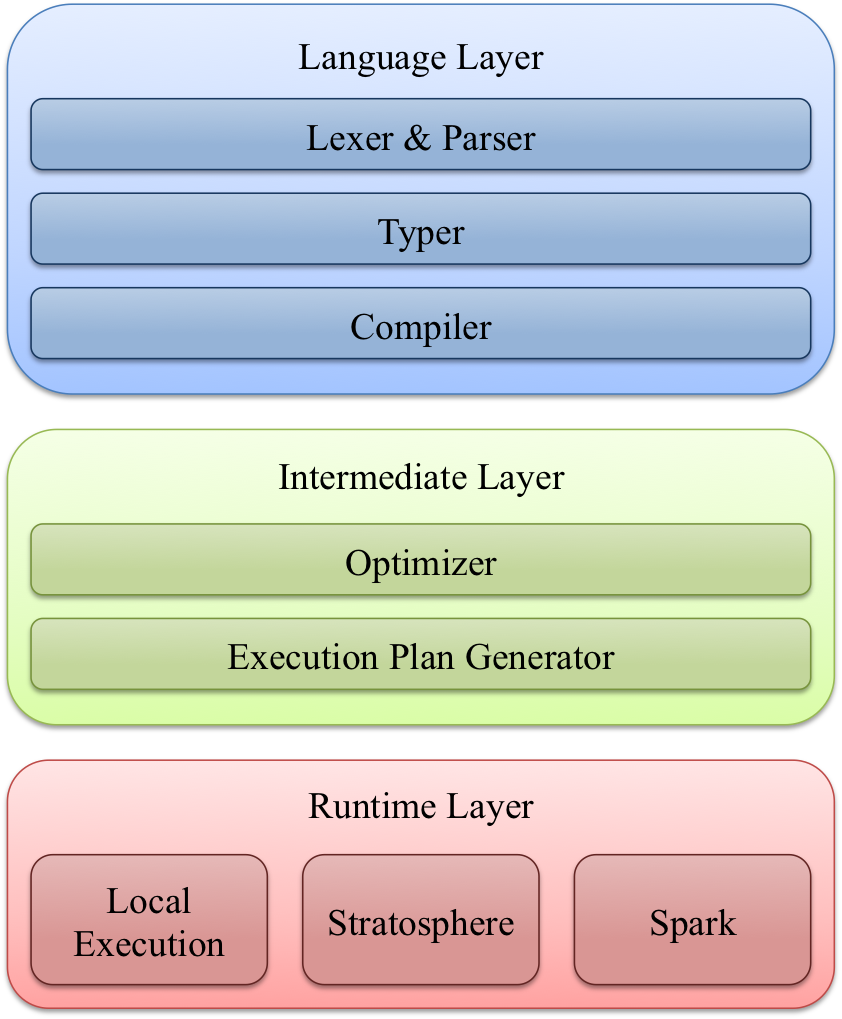
\includegraphics[height=0.175\paperheight]{images/systemArchitecture.png}
\caption{The layered system architecture of Gilbert. The language layer is responsible for parsing, typing and compiling the given Matlab code. The intermediate layer facilitates high-level optimization strategies. The runtime layer is responsible for executing the specified program in parallel.}
\label{fig:systemArchitecture}
\end{figure}

As a solution we propose Gilbert, a distributed sparse linear algebra environment. Gilbert provides a Matlab-like language for distributed sparse linear algebra operations. It has a layered architecture, which is shown in Figure \ref{fig:systemArchitecture}. The first layer is the language layer. It contains all functionality to parse the given Gilbert code and to compile it into an intermediate representation (IR). The second layer is the intermediate layer and it receives the IR of the Gilbert code. The intermediate format is the ideal representation to apply language independent high-level transformations. The Gilbert optimizer applies several algebraic optimizations prior to the generation of the execution plan. The execution plan generator translates the optimized IR into a specific execution plan, depending on the selected execution engine. Once the program has been translated into an execution engine's specific plan, it is executed on the respective back end. 

Our main contributions are:
\begin{itemize}
 \item Gilbert allows to write MATLAB-like code for sparse linear algebra and execute it on massively parallel dataflow systems.
 \item Its expressiveness allows to quickly develop scalable algorithms to analyze web-scale data.
 \item We introduce a novel fixed-point operator which replaces loops by recursion and can be efficiently parallelized.
 \item Furthermore, we demonstrate that dataflow optimizers can be used to automatically select an good matrix multiplication strategy. 
\end{itemize}
%Gilbert provides a Matlab-like language for distributed sparse linear algebra operations. %Being such a system, it comprises the complete stack of functionalities necessary to implement a programming language. At first, the system has to divide the given source code into tokens. These tokens are parsed and an abstract syntax tree (AST) is created. In order to generate the intermediate representation (IR), type information is needed for all expressions. This information is extracted by the typing system. Knowing the types, the compiler can translate the Gilbert program into its IR. The IR is well suited to apply high-level transformations to the program. At last, the execution plan generator translates the IR into an execution plan which can be executed in parallel. %The layered system architecture is shown in \cref{fig:systemArchitecture}. 

%%It has a layered architecture. The first layer is the language layer. It contains all functionality to parse the given Gilbert code and to compile it into an intermediate representation (IR). The second layer is the intermediate layer and it receives the IR of the Gilbert code. The intermediate format is the ideal representation to apply language independent high-level transformations. The Gilbert optimizer applies several algebraic optimizations prior to the generation of the execution plan. The execution plan generator translates the optimized IR into a specific execution plan, depending on the selected execution engine. Once the program has been translated into an execution engine's specific plan, it is executed on the respective back end.

%\begin{figure}[t!]
% \centering
% 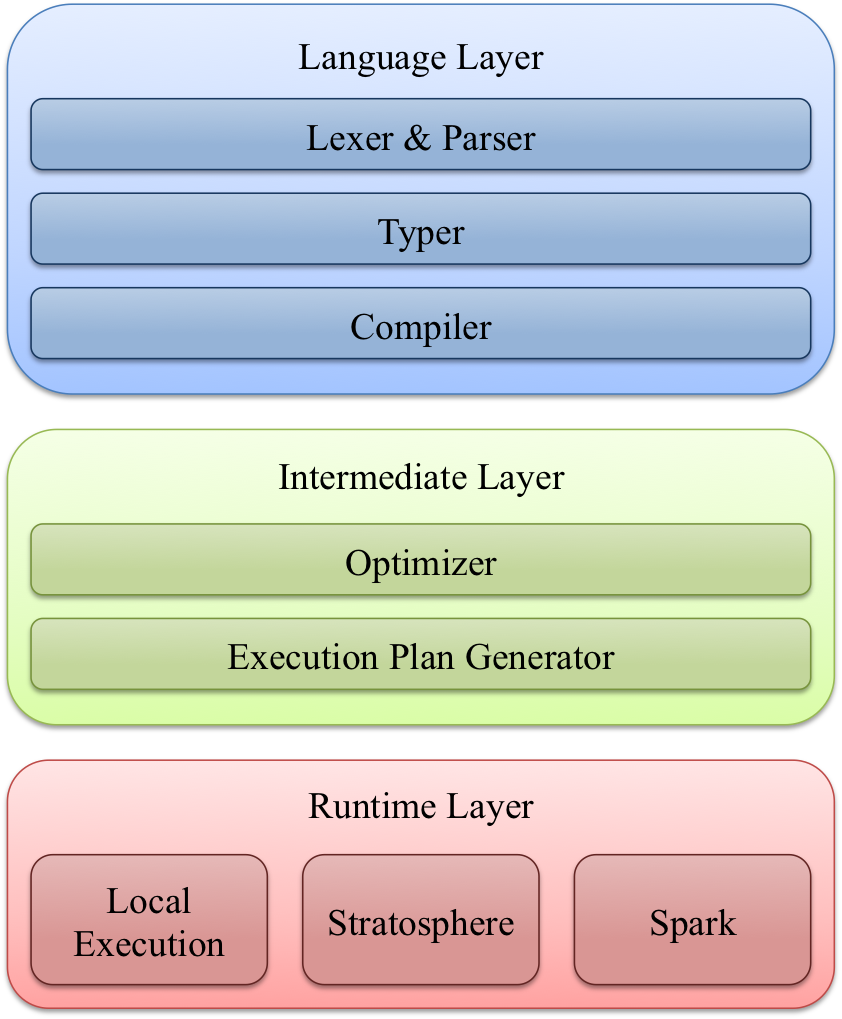
\includegraphics[height=0.175\paperheight]{images/systemArchitecture.png}
% \caption{The layered system architecture of Gilbert. The language layer is responsible for parsing, typing and compiling the given Matlab code. The intermediate layer facilitates high-level optimization strategies. The runtime layer is responsible for executing the specified program in parallel.}
% \label{fig:systemArchitecture}
%\end{figure}

%%\textbf{Language Layer}. The language layer contains all the logic for translating Gilbert source code into the intermediate representation, see the subsequent section for more details. %Gilbert's supported language and its features is described in \cref{sec:gilbertLanguage}.
%%The resulting AST is attributed with type information by the typing system. The typer makes use of the Hindley-Milner algorithm to automatically infer types.%, as it is described in~\cref{sec:hmInference}. 
%%The type information enriched AST is then translated into a front end independent representation of linear algebra operations, namely the IR. The format Gilbert uses to represent linear algebra operations in a generalized format is described in Section~\ref{sec:intermediaterepresentation}.

%%\textbf{Intermediate Layer}. The intermediate layer contains the optimizer and the execution plan generator. The optimizer applies the optimizations described in Section~\ref{sec:gilbertOptimizer} to IR of the Gilbert program. Then the IR is translated into the execution engine's specific format. The linear algebra operations are translated into a dataflow graph as explained in Section~\ref{sec:LinearAlgebraOperations}. The system supports Flink and Spark as parallel execution engines.

The rest of this paper is structured as follows. %In \ref{sec:overview} we give an overview of Gilbert.
%Then, 
In \Cref{sec:gilbertFeatures}, Gilbert's language and its features are described.
\Cref{sec:gilbertRuntime} presents how linear algebra operations are mapped to a dataflow system. Gilbert's performance and scalability is evaluated in \Cref{sec:evaluation}.
Related work is covered in \Cref{sec:relatedWork} before the work is concluded in \Cref{sec:conclusion}.
%%!TEX root=paper.tex
\section{Overview}
\label{cha:overview}

Gilbert provides a Matlab-like language for distributed sparse linear algebra operations.
Being such a system, it comprises the complete stack of functionalities necessary to implement a programming language.
At first, the system has to divide the given source code into tokens.
These tokens are parsed and an abstract syntax tree (AST) is created.
In order to generate the intermediate representation (IR), type information is needed for all expressions.
This information is extracted by the typing system.
Knowing the types, the compiler can translate the Gilbert program into its IR.
The IR is well suited to apply high-level transformations to the program.
At last, the execution plan generator translates the IR into an execution plan which can be executed in parallel.
The layered system architecture is shown in \cref{fig:systemArchitecture}.

\begin{figure}
	\centering
	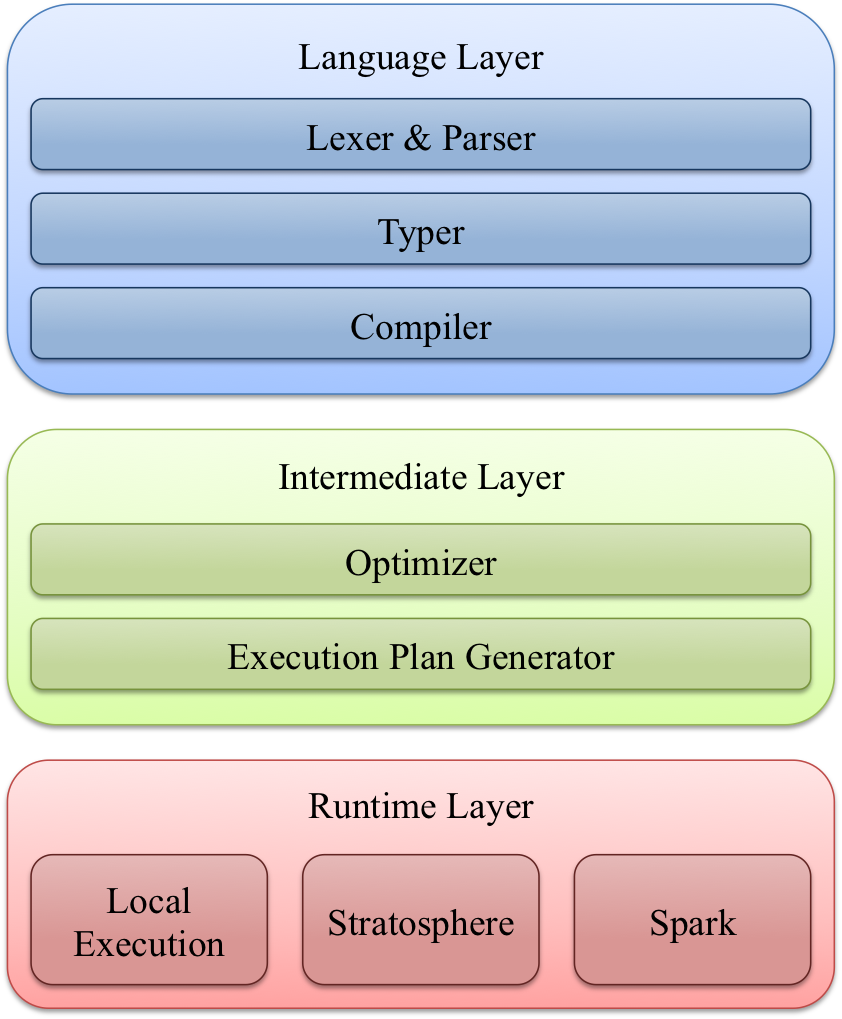
\includegraphics[height=0.175\paperheight]{images/systemArchitecture.png}
	\caption{The layered system architecture of Gilbert. The language layer is responsible for parsing, typing and compiling the given Matlab code. The intermediate layer facilitates high-level optimization strategies. The runtime layer is responsible for executing the specified program in parallel.}
	\label{fig:systemArchitecture}
\end{figure}

The first layer is the language layer.
It contains all functionality to parse the given Gilbert code and to compile it into the IR.
The second layer is the intermediate layer and it receives the IR of the Gilbert code.
The intermediate format is the ideal representation to apply language independent high-level transformations.
The Gilbert optimizer applies several algebraic optimizations prior to the generation of the execution plan.
The execution plan generator translates the optimized IR into a specific execution plan, depending on the selected execution engine.
Once the program has been translated into an execution engine's specific plan, it is executed on the respective back end.

\subsection{Language Layer}

The language layer contains all the logic for translating Gilbert source code into the intermediate representation, see \cref{cha:intermediaterepresentation} for more details.
Gilbert's supported language and its features is described in \cref{sec:gilbertLanguage}.

The resulting AST is attributed with type information by the typing system.
The typer makes use of the Hindley-Milner algorithm to automatically infer types, as it is described in \cref{sec:hmInference}.
The type information enriched AST is then translated into a front end independent representation of linear algebra operations, namely the IR.
The format Gilbert uses to represent linear algebra operations in a generalized format is described in \cref{cha:intermediaterepresentation}.

\subsection{Intermediate Layer}

The intermediate layer contains the optimizer and the execution plan generator.
The optimizer applies the optimizations described in \cref{cha:optimizer} to IR of the Gilbert program.
Then the IR is translated into the execution engine's specific format.
The linear algebra operations are translated into a dataflow graph as explained in \cref{sec:operatorImplementation}.
The system supports Flink and Spark as parallel execution engines.
%!TEX root=paper.tex
\section{Gilbert Features}
\label{sec:gilbertFeatures}

Gilbert's language has been strongly inspired by MATLAB, which should ease its adoption.
The language is a fully functional subset of MATLAB and its grammar is specified in \cite{Rohrmann2014}.
The elementary data type is the matrix. 
Gilbert supports arbitrary $2$-dimensional matrices whose elements can be \emph{double} or \emph{boolean}.
Vectors are not represented by a special type but instead are treated as a single column/row matrix.
Additionally, scalar \emph{double}, \emph{boolean}, and \emph{string} values are supported. 
Gilbert also implements cell array types.
A cell array is defined using curly braces and commas to separate individual values. 
The cells can be accessed by an index appended in curly braces to the cell array variable. 
\Cref{lst:cellArray} shows how to define and access them.
\begin{listing}[!h]
    \begin{lstlisting}[language=Matlab,
        commentstyle=\color{black},
        stringstyle=\color{black},
        xleftmargin=.2\textwidth,
        basicstyle=\small
    ]
c = {true, 2*2, 'cell', 'array'};
b = c{1} & false; % = false
d = c{2} ^ 2; % = 16
s = {c{4}, c{3}}; % = {'array', 'cell'} 
    \end{lstlisting}
  \caption{Cell array usage in Gilbert. Definition of a 4 element cell array, which is accessed subsequently.}
  \label{lst:cellArray}
\end{listing}

Gilbert supports the basic linear algebra operations defined on matrices and scalars. 
They include among others \code{+}, \code{-}, \code{/}, and \code{*}, whereas \code{*} denotes the matrix-matrix multiplication and all other operations are interpreted cell-wise. 
The cell-wise multiplication is indicated by a point preceding the operator. 
Gilbert also supports comparisons operators such as \code{>}, \code{>=}, \code{==}, and \code{\textasciitilde=}. 
Besides the basic arithmetic operations, the user can also define named functions and anonymous functions. 
The syntax of anonymous functions adheres to the MATLAB syntax: \code{@(x,y) x*x + y*y}. 

An important aspect of MATLAB are loops. 
MATLAB permits the user to express \code{for} and \code{while} loops, which can have side effects. 
Parallelizing iterations with side effects is difficult because the referenced external state has to be maintained. 
This circumstance makes preprocessing and execution unnecessarily complex. 
Gilbert offers a fixpoint operator \code{fixpoint}, which iteratively applies a given update function $f$ on the previous result of $f$, starting with an initial value $x$ at iteration $0$.
\small
\begin{displaymath}
  n^{th}\text{ iteration}\equiv\underbrace{f(f(\ldots(f(x))\ldots))}_{\text{$n$ times}}
\end{displaymath}
\normalsize

In order to terminate the fixpoint operation, the operator provides two mechanisms.
The user has to specify a maximum number \code{m} of iterations.
Additionally, the user can provide a convergence function \code{c} to the fixpoint operator.
The convergence function is called with the previous and current fixpoint value and returns a boolean value.
Thus, the fixpoint operator terminates either if convergence was detected or if the maximum number of iterations is exceeded.
\small
\begin{equation}
\label{eq:fixpoint}
fixpoint: \underbrace{T}_{\text{\code{x}}} \times \left( \underbrace{T \rightarrow T}_{\text{\code{f}}} \right) \times \underbrace{\mathbb{N}}_{\text{\code{m}}} \times \left(\underbrace{T\times T \rightarrow \mathbb{B}}_{\text{\code{c}}} \right) \rightarrow T
\end{equation}
\normalsize
with $T$ being a generic type variable.

In fact, the fixpoint operator replaces iterations by recursions with a pure update function $f$. 
At this point Gilbert breaks with existing MATLAB code. 
However, all MATLAB loops can be expressed via the fixpoint operator by passing the loop's closure to the update function, see \cref{fig:for2Fixpoint}.
\begin{listing}[!h]
  \centering
  \begin{sublisting}{.4\linewidth}
    \begin{lstlisting}[language=Matlab,
      commentstyle=\color{black},
      stringstyle=\color{black},
      keywordstyle=\color{black}\bfseries,
      basicstyle=\small
    ]
A = 0;
for i = 1:10
  A = A + i;
end
    \end{lstlisting}
    \caption{For loop}
    \label[listing]{fig:for2Fixpoint:for}
  \end{sublisting}
  \begin{sublisting}{.5\linewidth}
      \begin{lstlisting}[language=Matlab, basicstyle=\footnotesize]
f = @(x) ...
  {x{1} + x{2}, x{2} + 1};
r = fixpoint({0,1}, f, 10);
A = r{1};
    \end{lstlisting}
    \caption{Fixpoint}
    \label[listing]{fig:for2Fixpoint:fixpoint}
  \end{sublisting}
  \caption{Transformation from MATLAB for loop \subref{fig:for2Fixpoint:for} to Gilbert fixpoint \subref{fig:for2Fixpoint:fixpoint} formulation. Essentially, all iteration data is combined and passed as a cell array value to the update function.}
  \label{fig:for2Fixpoint}
\end{listing}

\subsection{Gilbert Typing System}
\label{sec:gilberttyping}

MATLAB belongs to the class of dynamically typed languages.
However, the parallel data processing systems used to run Gilbert programs need to know the occurring data types.
Therefore, the MATLAB language has to be enriched with type information. 
We infer this type information using the Hindley-Milner (HM) type system~\cite{hindley:tams1969a,milner:jcss1978a} and a slightly derived form of algorithm W~\cite{damas:1982a} for type inference. 
In case that the type inference algorithm cannot properly infer the types, there has to be a way to resolve this problem. 
Similar to \cite{furr:2009a}, we allow to add type information via special comments.

\textbf{Function Overloading}. MATLAB's basic operators, such as \code{+}, \code{-}, \code{/} and \code{*}, for example, are overloaded.
They can be applied to matrices, scalars as well as mixture of both data types.
That makes it very convenient to express mathematical problems, but from a programmer's point of view it causes some hardships.
Originally, HM cannot deal with overloaded functions, because it assumes that each function has a unique type.
In order to extend HM's capabilities, we allowed each function symbol to have a list of signatures.
In the case of \code{+}, the list of signatures would consist of 
\small
\begin{alignat*}{2}
matrix[double] \times matrix[double] &\rightarrow matrix[double]\\
matrix[double] \times double &\rightarrow matrix[double]\\
double \times matrix[double] &\rightarrow matrix[double]\\
double \times double &\rightarrow double
\end{alignat*}
\normalsize

In order to solve the typing problem, the inference algorithm has to resolve this ambiguity.
Having complete knowledge of the argument types is enough to select the appropriate signature.
Sometimes even partial knowledge is sufficient.

\textbf{Matrix Size Inference}. Matrices constitute the elementary data type in our linear algebra environment.
Besides its element type, a matrix is also defined by its size.
In the context of program execution, knowledge about matrix sizes can help to optimize the evaluation.
For instance, consider a threefold matrix multiplication $A\times B\times C$.
The multiplication can be evaluated in two different ways: $(A\times B)\times C$ and $A\times(B\times C)$.
For certain matrix sizes one way might be infeasible whereas the other way can be calculated efficiently due to the matrix size of the intermediate result $(A\times B)$ or $(B\times C)$.

By knowing the matrix sizes, Gilbert can choose the most efficient strategy to calculate the requested result.
Another advantage is that we can decide whether to carry out the computation in-core or in parallel depending on the matrix sizes.
Sometimes the benefit of parallel execution is smaller than the initial communication overhead and thus it would be wiser to execute the calculation locally.
Furthermore, it can be helpful for data partitioning on a large cluster and to decide on a blocking strategy with respect to the algebraic operations.
Therefore, we extended the HM type inference to also infer matrix sizes where possible.

Gilbert's matrix type is defined as 
\small
\begin{displaymath}
MatrixType(\underbrace{\tau}_{\text{Element type}},\underbrace{\nu}_{\text{Number of rows}},\underbrace{\nu}_{\text{Number of columns}})
\end{displaymath}
\normalsize
with $\nu$ being the value type. The value type can either be a value variable or a concrete value.

The matrix size inference is incorporated into the HM type inference by adapting the \code{unify} function.
Whenever we encounter a matrix type during the unification process, we call a \code{unifyValue} function on the two row and column values.
The \code{unifyValue} function works similarly to the \code{unify} function.
First, the function resolves the value expression, thus substituting value variables with their assigned values.
Then, if at least one of the resolved value expressions is still a value variable, then the union is constructed and the corresponding value variable dictionary entry is updated.
If both resolved expressions are equal, then this value is returned. 
Otherwise an error is thrown.

\subsection{Intermediate Representation}
\label{sec:intermediaterepresentation}

After parsing and typing of the source code is done, it is translated into an intermediate representation. 
The additional abstraction layer allows Gilbert to apply language independent optimization.
Moreover, the higher-level abstraction of mathematical operations holds more potential for algebraic optimization. 
The intermediate format consists of a set of operators to represent the different linear algebra operations. 
Every operator has a distinct result type and a set of parameters which are required as inputs. 
The set of intermediate operators can be distinguished into three categories: \emph{Creation operators}, \emph{transformation operators} and \emph{output operators}.

\textbf{Creation Operators}. Creation operators generate or load some data.
The \code{load} operator loads a matrix from disk with the given number of rows and columns.
The \code{eye} operator generates an identity matrix of the requested size.
\code{zeros} generates a matrix of the given size which is initialized with zeros.
\code{Randn} takes the size of the resulting matrix and the mean and the standard deviation of a Gauss distribution.
The Gauss distribution is then used to initialize the matrix randomly.

\textbf{Transformation Operators}. The transformation operators constitute the main abstraction of the linear algebra operations.
They group operations with similar properties and thus allow an easier reasoning and optimization of the underlying program. 
The \code{UnaryScalar\-Transformation} takes a single scalar value and applies an unary operation on it. 
The \code{ScalarScalarTransformation} constitutes a binary operation on scalar values whereas \code{ScalarMatrixTransformation} and \code{MatrixScalarTransformation} represent a binary operation between a scalar and a matrix value. 
The \code{VectorwiseMatrixTrans\-formation} applies an operation on each row vector of the given matrix.
A vectorwise operation produces a scalar value for each row vector. 
The \code{AggregateMatrixTransformation} applies an operation to all matrix entries producing a single scalar result value. 
The iteration mechanism is represented by the \code{Fixpoint\-IterationMatrix} and \code{FixpointIteration\-CellArray} operators. 

\textbf{Writing Operators}. The writing operators are used to write the computed results back to disk.
There exists a writing operation for each supported data type: \code{WriteMatrix}, \code{WriteScalar}, \code{WriteString}, \code{WriteCellArray} and \code{WriteFunction}.

\subsection{Gilbert Optimizer}
\label{sec:gilbertOptimizer}

The Gilbert optimizer applies algebraic optimizations to a Gilbert program.
The optimizer exploits equivalence transformations which result from the commutative and associative properties of linear algebra operations.
It works on the intermediate format of a program, which provides an appropriate high-level abstraction.

\textbf{Matrix Multiplication Reordering}. Matrix multiplications belong to the most expensive linear algebra operations in terms of computational as well as space complexity. 
Intermediate results of successive matrix multiplications can easily exceed the memory capacity and thus rendering its computation infeasible. However, a smart execution order can sometimes avoid the materialization of excessively large matrices. 
The best execution order of successive multiplications is the one that minimizes the maximum size of intermediate results.
In order to determine the best execution order, the optimizer first extracts all matrix multiplications with more than $2$ operands.
Then, it calculates the maximum size of all occurring intermediate results for each evaluation order.
In order to do this calculation, the optimizer relies on the operands' automatically inferred matrix sizes.
At last, it picks the execution order with the minimal maximum intermediate matrix size.

\textbf{Transpose Pushdown}. Transpose pushdown tries to move the transpose operations as close to the matrix input as possible.
Thereby, consecutive transpose operations accumulate at the inputs and unnecessary operations erase themselves.
Consider, for example, $C = A^TB$ and $E = (CD^T)^T$.
By inserting $C$ into $E$, the expression $E=(A^T BD^T)^T$ is obtained which is equivalent to $DB^T A$. 
The latter formulation contains only one transpose operation. 
Usually multiple transpose operations occur because they are written for convenience reasons at various places in the code. 
Moreover, in complex programs it is possible that the programmer loses track of them or simply is unaware of the optimization potential. 
Therefore, transpose pushdown can be a beneficial optimization.
%!TEX root=main.tex
\section{Gilbert Runtime}
\label{sec:gilbertRuntime}

The Gilbert runtime is responsible for executing the compiled MATLAB code on a particular platform. For this purpose, it receives the intermediate representation of the code and translates it into the execution engine's specific format. Currently, Gilbert supports three different execution engines: \emph{ReferenceExecutor}, \emph{FlinkExecutor} and \emph{SparkExecutor}. The \emph{ReferenceExecutor} executes the compiled MATLAB code locally. For the distributed execution Gilbert supports the Spark and the Flink system as backends. The \emph{ReferenceExecutor} is an interpreter for the intermediate code.
It takes the dependency tree of a MATLAB program and executes it by evaluating the operators bottom-up. In order to evaluate an operator, the system first evaluates all inputs of an operator and then executes the actual operator logic. Since the program is executed locally, the complete data of each operator is always accessible and, thus, no communication logic is required. All input and output files are directly written to the local hard drive. In contrast to the \emph{ReferenceExecutor}, the \emph{FlinkExecutor} executes the program in parallel. It takes the dependency tree of a MATLAB program and translates it into a PACT plan. After the plan is generated, it is issued to the Flink system for parallel execution. This approach implies that the program is not directly executed by the executor. Instead, the executor represents just another translation step. The PACT plans are executed in parallel. Consequently, data structures are needed which can be distributed across several nodes and represent the commonly used linear algebra abstractions, such as vectors and matrices. Moreover, the linear algebra operations have to be adjusted so that they keep working in a distributed environment. Fortunately, Flink offers a rich and expressive API to easily realize distributed computations. The details of the distributed data structures and operations are explained in \cref{sec:DistributedMatrixRepresentation} and \cref{sec:LinearAlgebraOperations}. The \emph{SparkExecutor} is the second executor for distributed computations. In contrast to the \emph{FlinkExecutor}, it executes the MATLAB programs on top of the Spark system. Since Spark and Flink offer a similar set of programming primitives, they can both operate on the same data structures. Furthermore, even most of the linear algebra operations can be implemented similarly.

\subsection{Distributed Matrix Representation}
\label{sec:DistributedMatrixRepresentation}

One aspect of writing distributed algorithms is how the relevant data is distributed across several worker nodes. Since the distribution pattern directly influences the algorithms, one cannot consider them independently from one another. In Gilbert's use case, the main data structure are matrices. Thus, a partitioning for matrices has to be conceived which allows efficient algorithms working on the distributed data. Looking at a matrix, one easily finds a multitude of different partition schemes. A first idea could be to partition a matrix according to their rows or columns, as it is depicted in \cref{fig:rowPartitioning} and \cref{fig:columnPartitioning}. This scheme allows to represent a matrix as a set of vectors which is stored in a distributed fashion.
Furthermore, it allows an efficient realization of cellwise operations, such as $+,-,/$ or $.*$. In order to calculate the result of such an operation, we only have to join the corresponding rows of both operands and execute the operation locally for each pair of rows.

\begin{figure}
	\centering
	\begin{subfigure}{.3\linewidth}
		\centering
		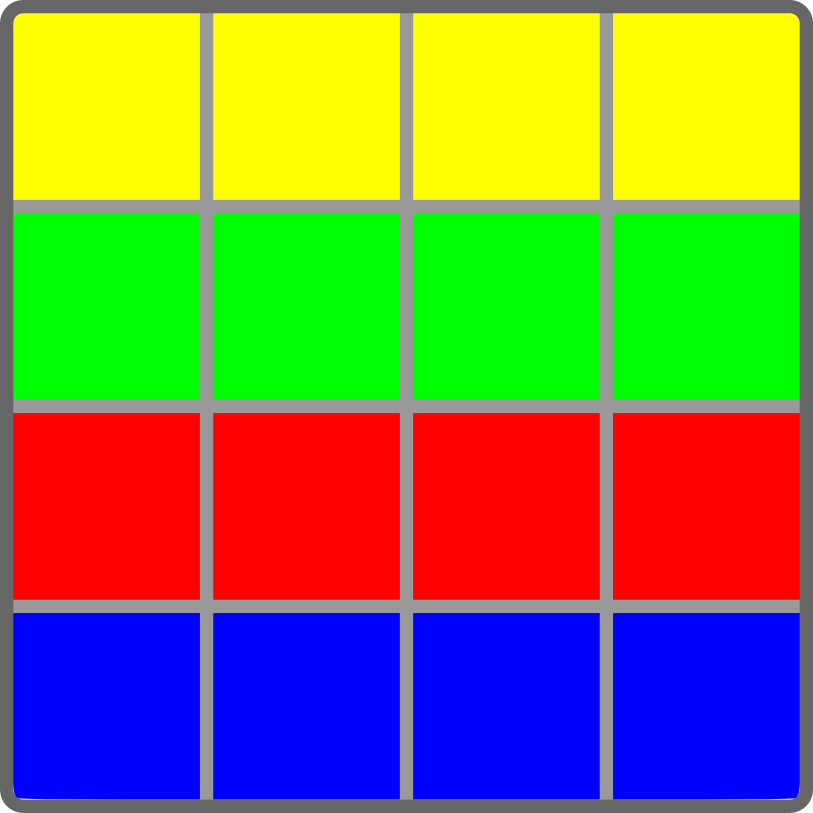
\includegraphics[width=0.55\textwidth]{images/rowPartitioning.png}
		\caption{Row partitioning}
		\label{fig:rowPartitioning}
	\end{subfigure}
	\begin{subfigure}{.3\linewidth}
		\centering
		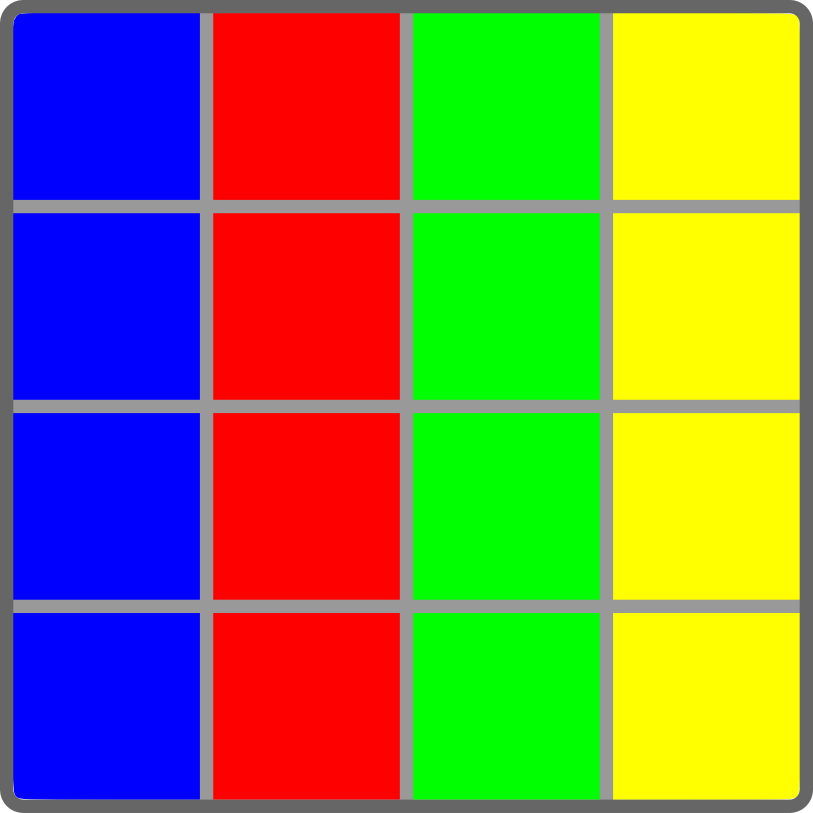
\includegraphics[width=0.55\textwidth]{images/columnPartitioning.png}
		\caption{Column partitioning}
		\label{fig:columnPartitioning}
	\end{subfigure}
	\begin{subfigure}{.3\linewidth}
		\centering
		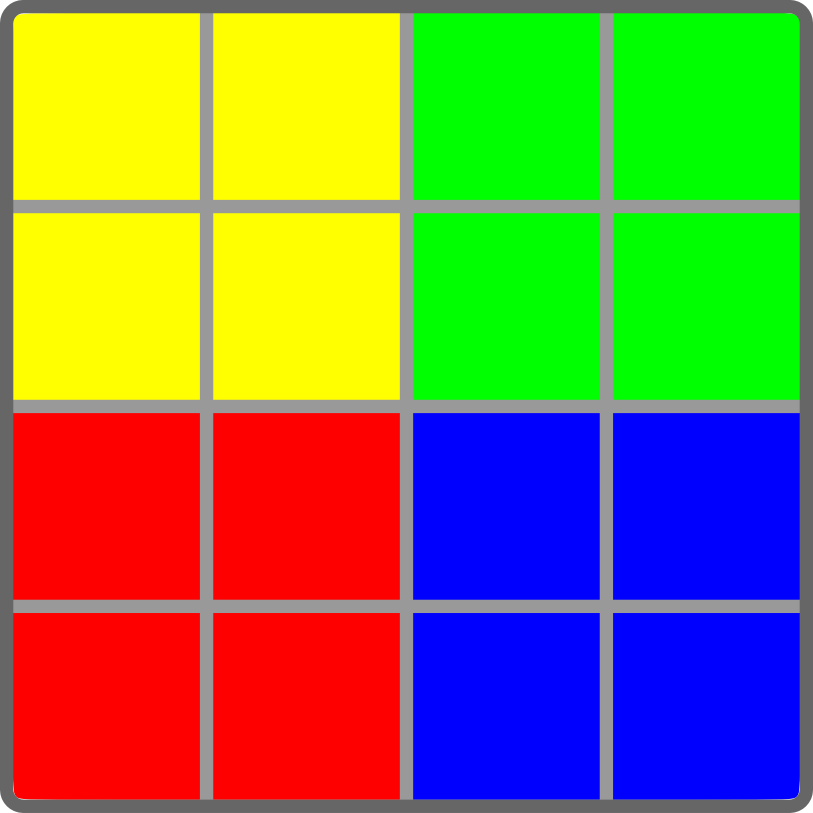
\includegraphics[width=0.55\textwidth]{images/quadraticBlockPartitioning.png}
		\caption{Square block partitioning}
		\label{fig:quadraticBlockPartitioning}
	\end{subfigure}
	\caption{Row-wise, column-wise and square block-wise matrix partitioning.}
	\label{fig:Partitionings}
\end{figure}

However, this approach unveils its drawbacks when multiplying two equally partitioned matrices $A$ and $B$. In such a case, the row $r$ of $A$ and the complete matrix $B$ is needed to calculate the resulting row with index $r$. This circumstance implies a complete repartitioning of $B$. The repartitioning is especially grave, since $B$ has to be broadcasted to every row of $A$. In order to quantify the repartitioning costs of such a matrix multiplication, a simple cost model is developed. First of all, it is limited to modeling the communication costs, since network I/O usually constitutes the bottleneck of distributed systems and is thus the dominating factor. For the sake of simplicity, the multiplication of two quadratic matrices $A \in \mathbb{R}^{n\times n}$ and $B \in \mathbb{R}^{n\times n}$ giving the matrix $C\in \mathbb{R}^{n \times n}$ is considered. Moreover, we assume that there are $n$ worker nodes available, each of which receiving a single row of $A$ and $B$, respectively. Thus, $A$ and $B$ are row-wise partitioned. We further assume that rows with the same index are kept on the same worker node. Each row $a_r$ requires the complete knowledge of matrix $B$ in order to produce the row $c_r$. Therefore, every row $b_r$ has to be sent to all other worker nodes. Thus, the number of rows sent by each worker node is $n-1$. All of the $n$ worker nodes have to do the same. Consequently, the total number of sent messages is $n(n-1)$ and each message has a size of $n\alpha$ where $\alpha$ is the size of a matrix entry. Usually, each sending operation causes some constant overhead inflicted by resource allocation. Before sending the actual data over the network, memory to transfer the data to the network interface has to be allocated, network resources have to be reserved and a network connection with the remote peer has to be established. This overhead is denoted by $\Delta$. Since all sending operations occur in parallel, the costs caused by constant overhead are $(n-1)\Delta$. The total amount of data, which has to sent over the network, is $n^2(n-1)\alpha$. The network interconnection is assumed to guarantee every node a bandwidth $\nu$. Therefore, the time needed for sending the data is $\frac{n^2(n-1)\alpha}{\nu}$. These considerations lead to the following repartitioning cost model:
\begin{displaymath}
	cost_{row} = \frac{n^2(n-1)\alpha}{\nu} + (n-1)\Delta
\end{displaymath}
Row and column partitioning are extreme forms of blocking. A less extreme form would be to split the matrix into equally sized quadratic blocks as shown in \cref{fig:quadraticBlockPartitioning}. In order to identify the individual blocks, each of them will be assigned a block row and block column index assigned. Thus, blocking adds some memory overhead in the form of index information. The blocks are distributed across the worker nodes. The block size directly controls the granularity of the partitioning. Increasing the block size will reduce the memory overhead of distributed matrices while reducing the degree of parallelism. Thus, the user has to adjust the block size value depending on the matrix sizes and the number of available worker nodes in order to obtain best performance. The quadratic block partitioning has similar properties like the row- and column-wise partitioning scheme when it comes to cellwise operations. We simply have to join corresponding blocks with respect to the pair of block row and column index and execute the operation on matching blocks locally. But how does this pattern performs for matrix multiplications? The assumptions are the same as before and additionally it is assumed that $n$ is a square number. Since the matrices $A$, $B$ and $C$ are equally partitioned into square blocks, indices will henceforth reference the block and not the matrix entry. In order to calculate the block $c_{ij}$, we have to know the block row $a_{i}$ and the block column $b_{j}$. The resulting block will be stored on the node $n_{ij}$ which already contains the blocks $a_{ij}$ and $b_{ij}$. Thus, each node $n_{ij}$ has to receive the missing $2\left(\sqrt{n}-1\right)$ blocks from the block row $a_{i}$ and block column $b_{j}$. In total, all worker nodes have to send $2n\left(\sqrt{n}-1\right)$ blocks. Each block has the size $n\alpha$. The total communication costs comprises the transmission costs and the network overhead:
\begin{displaymath}
	cost_{squareBlock} = \frac{2n^2\left(\sqrt{n}-1\right)\alpha}{\nu} + 2\left(\sqrt{n}-1\right)\Delta
\end{displaymath}
We see that the term $(n-1)$ is replaced by $2\left(\sqrt{n}-1\right)$ in the square block cost model. For $n>2$, the square block partitioning scheme is thus superior to the row- and column-wise partitioning pattern with respect to the cost model. The reason for this outcome is that the square blocks promote more localized computations compared to the other partitionings. Instead of having to know the complete matrix $B$, we only have to know one block row of $A$ and one block column of $B$ to compute the final result. Due to these advantages and also considering its simplicity, we decide to implement the square block partitioning scheme in Gilbert. It would also be possible to combine different partitionings and select them dynamically based on the data sizes and input partitionings. Besides the partitioning, Gilbert also has to represent the individual matrix blocks. There exist several storing schemes for matrices depending on the sparsity of the matrix. For example, if a matrix is dense, meaning that it does not contain many zero elements, the elements are best stored in a continuous array. If a matrix is sparse, then a hash map or some form of compressed representation are best suited. Gilbert chooses the representation of each block dynamically. Depending on the non-zero elements to total elements ratio, a sparse or dense representation is selected.

\subsection{Linear Algebra Operations}
\label{sec:LinearAlgebraOperations}

In the following, we will outline the implementation of the matrix multiplication operator (which is most critical for performance in linear algebra programs) in Gilbert as an example. For a reference of the implementation of the remaining operators, we refer the interested reader to~\cite{Rohrmann2014}. Note that we use the Breeze~\cite{breeze} library for conducting local in-operator linear algebraic operations. In a MapReduce-like system there exist two distinct matrix multiplication implementations for square blocking. The first approach is based on replicating rows and columns of the operands and is called replication based matrix multiplication (RMM). The other method is derived from the outer product formulation of matrix multiplications. It is called cross product based matrix multiplication (CPMM). The RMM and CPMM methods have been implemented within SystemML~\cite{ghoting:2011a}. Let us assume that we want to calculate $A \times B = C$ with $A,B$ and $C$ being matrices. The block size has been chosen such that $A$ is partitioned into $m\times l$ blocks, $B$ is partitioned into $l \times n$ blocks and the result matrix $C$ will be partitioned into $m\times n$ blocks. In order to reference the block in the $i$th block row and $j$th block column of $A$, we will write $A_{ij}$. A block row will be denoted by a single subscript index and a block column by a single superscript index. For example, $A_i$ marks the $i$th block row of $A$ and $A^j$ the $j$th block column of $A$. The replication-based strategy will copy for each $C_{ij}$ the $i$th block row of $A$ and the $j$th block column of $B$. The replicated blocks of $A_i$ and $B^j$ will be grouped together. These steps can be achieved by a single mapper. Once this grouping is done, the final result $C_{ij}$ can be calculated with a single reducer. The reduce function simply has to calculate the scalar product of $A_i$ and $B^j$. It is important to stress that $A_i$ is replicated for each $C_{ik},\forall k$. The whole process is illustrated in \cref{fig:RMM}.

\begin{figure}[h!]
	\centering
	\begin{subfigure}{.43\linewidth}
		\centering
		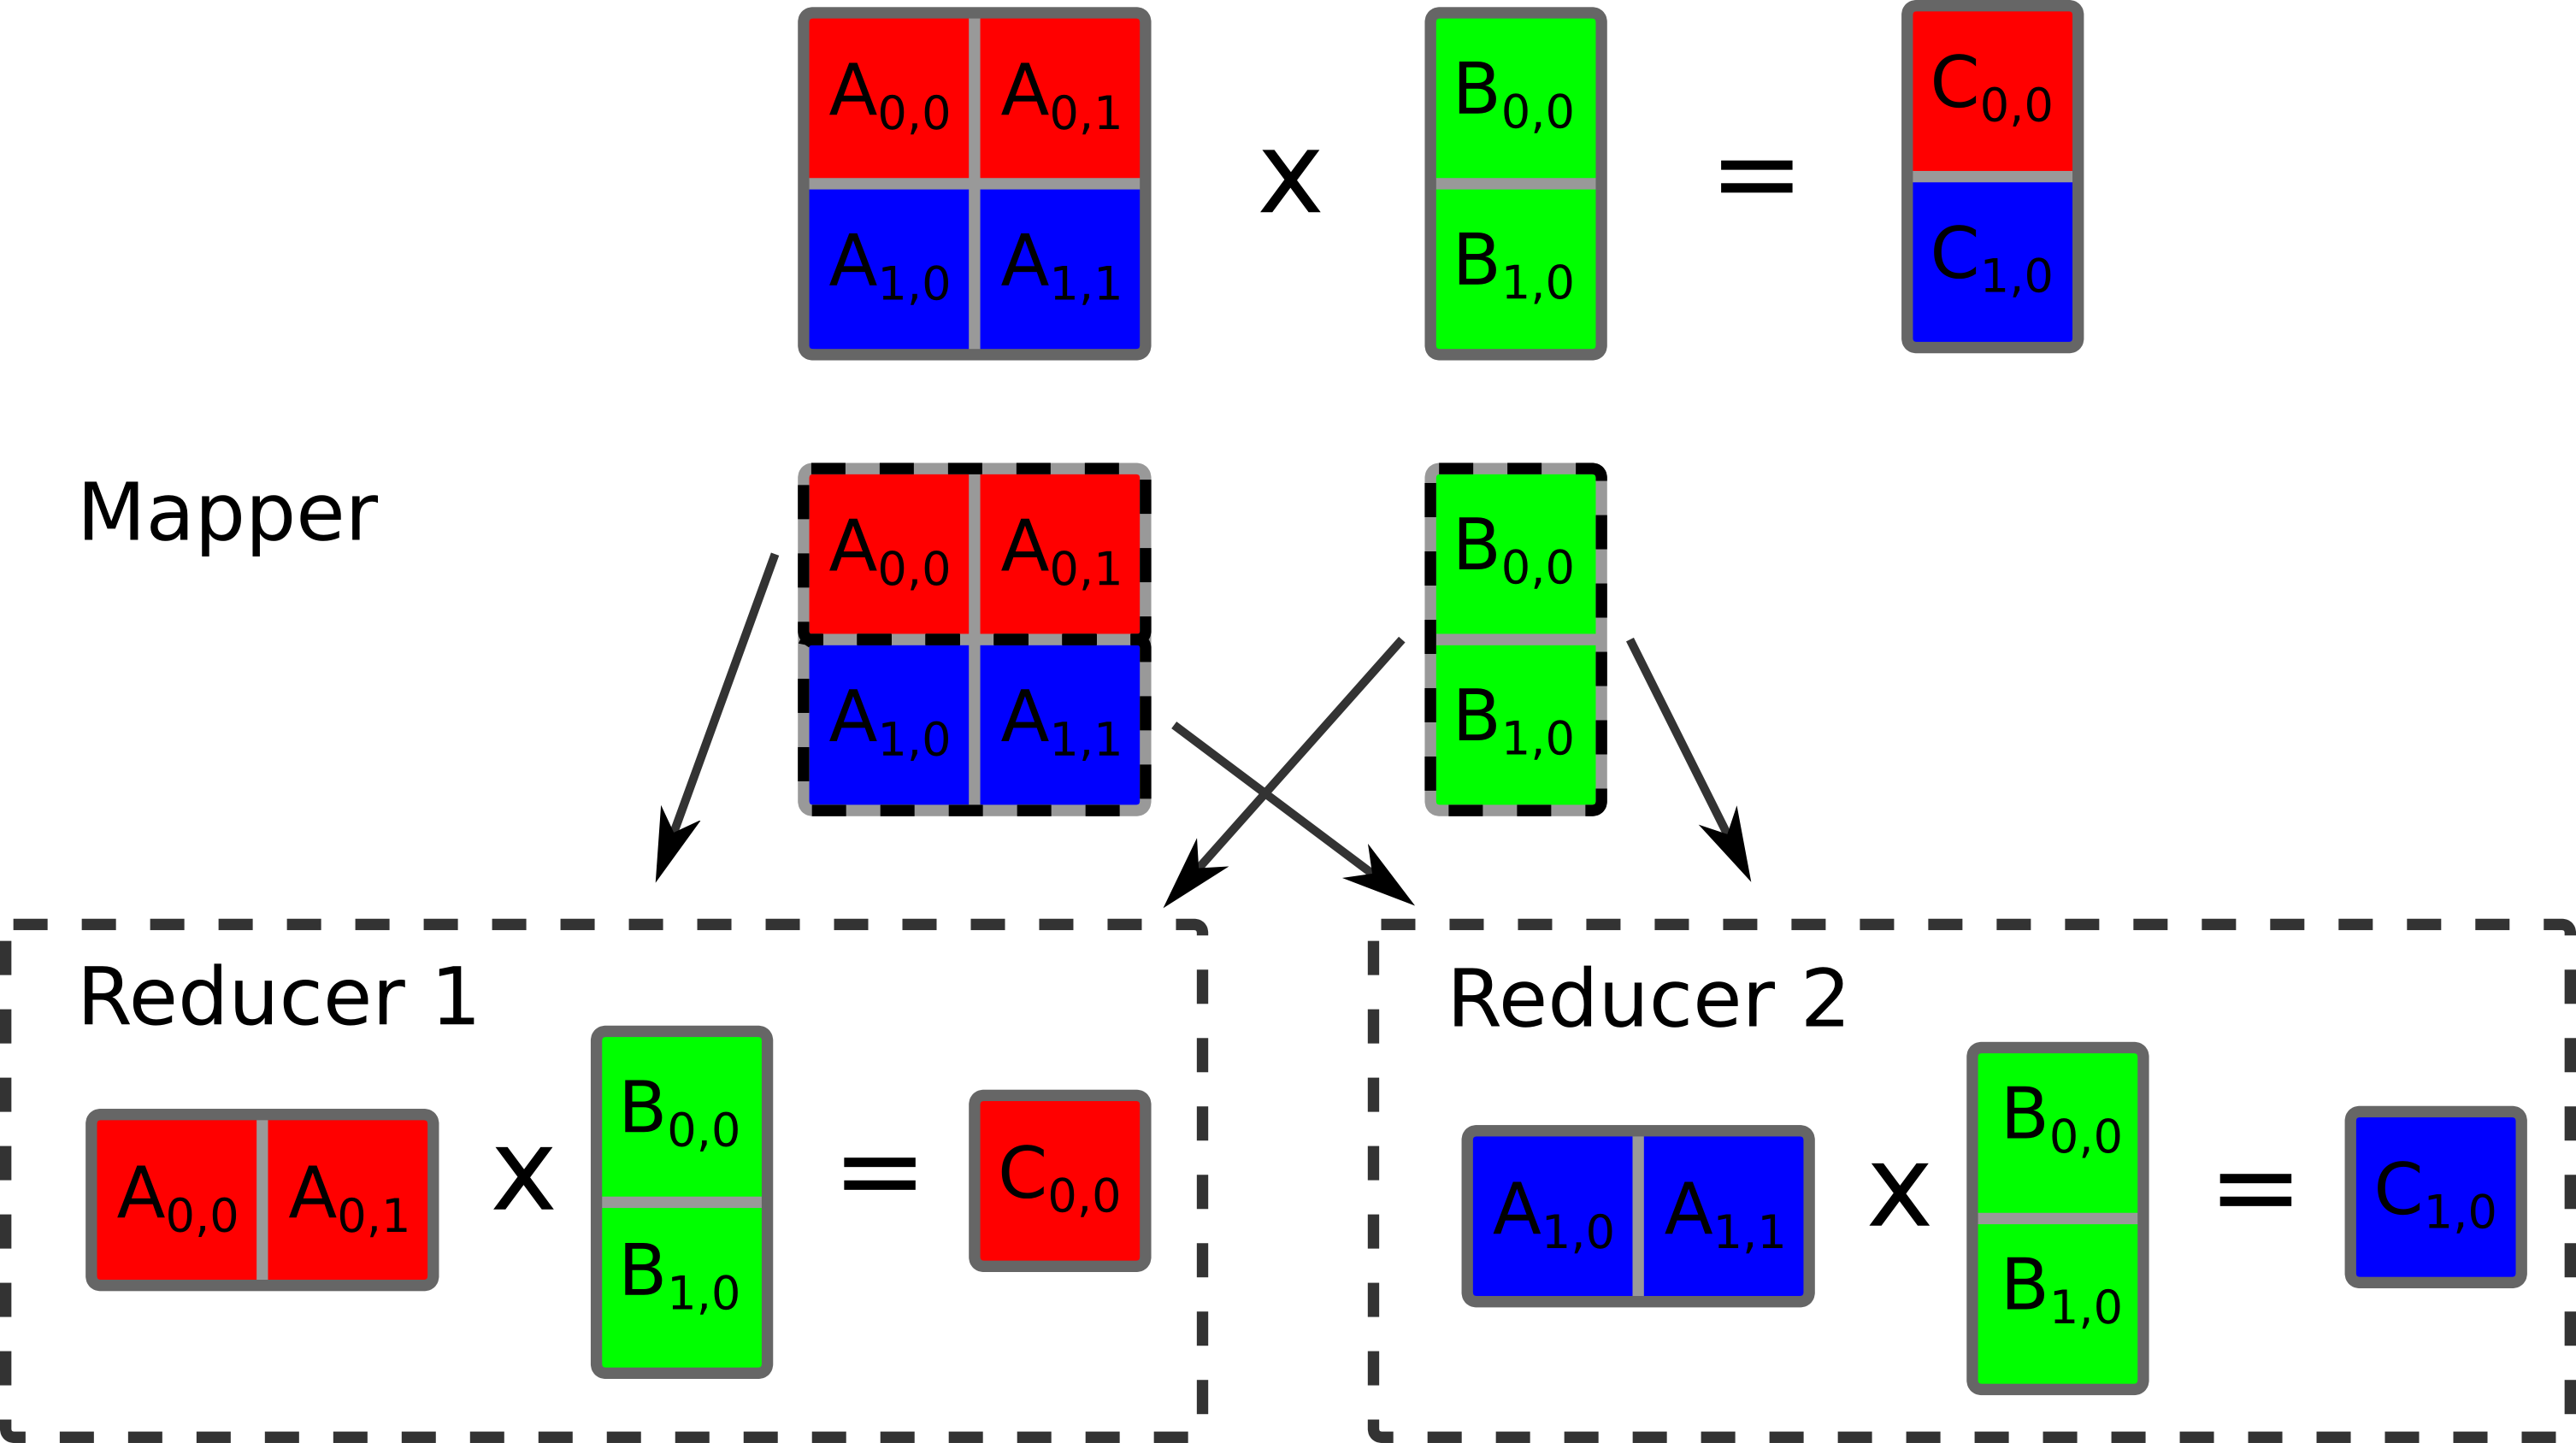
\includegraphics[width=0.99\linewidth]{images/rmm.png}
		\caption{Replication based matrix multiplication.}
		\label{fig:RMM}
	\end{subfigure}
	\hfill
	\begin{subfigure}{.43\linewidth}
		\centering
		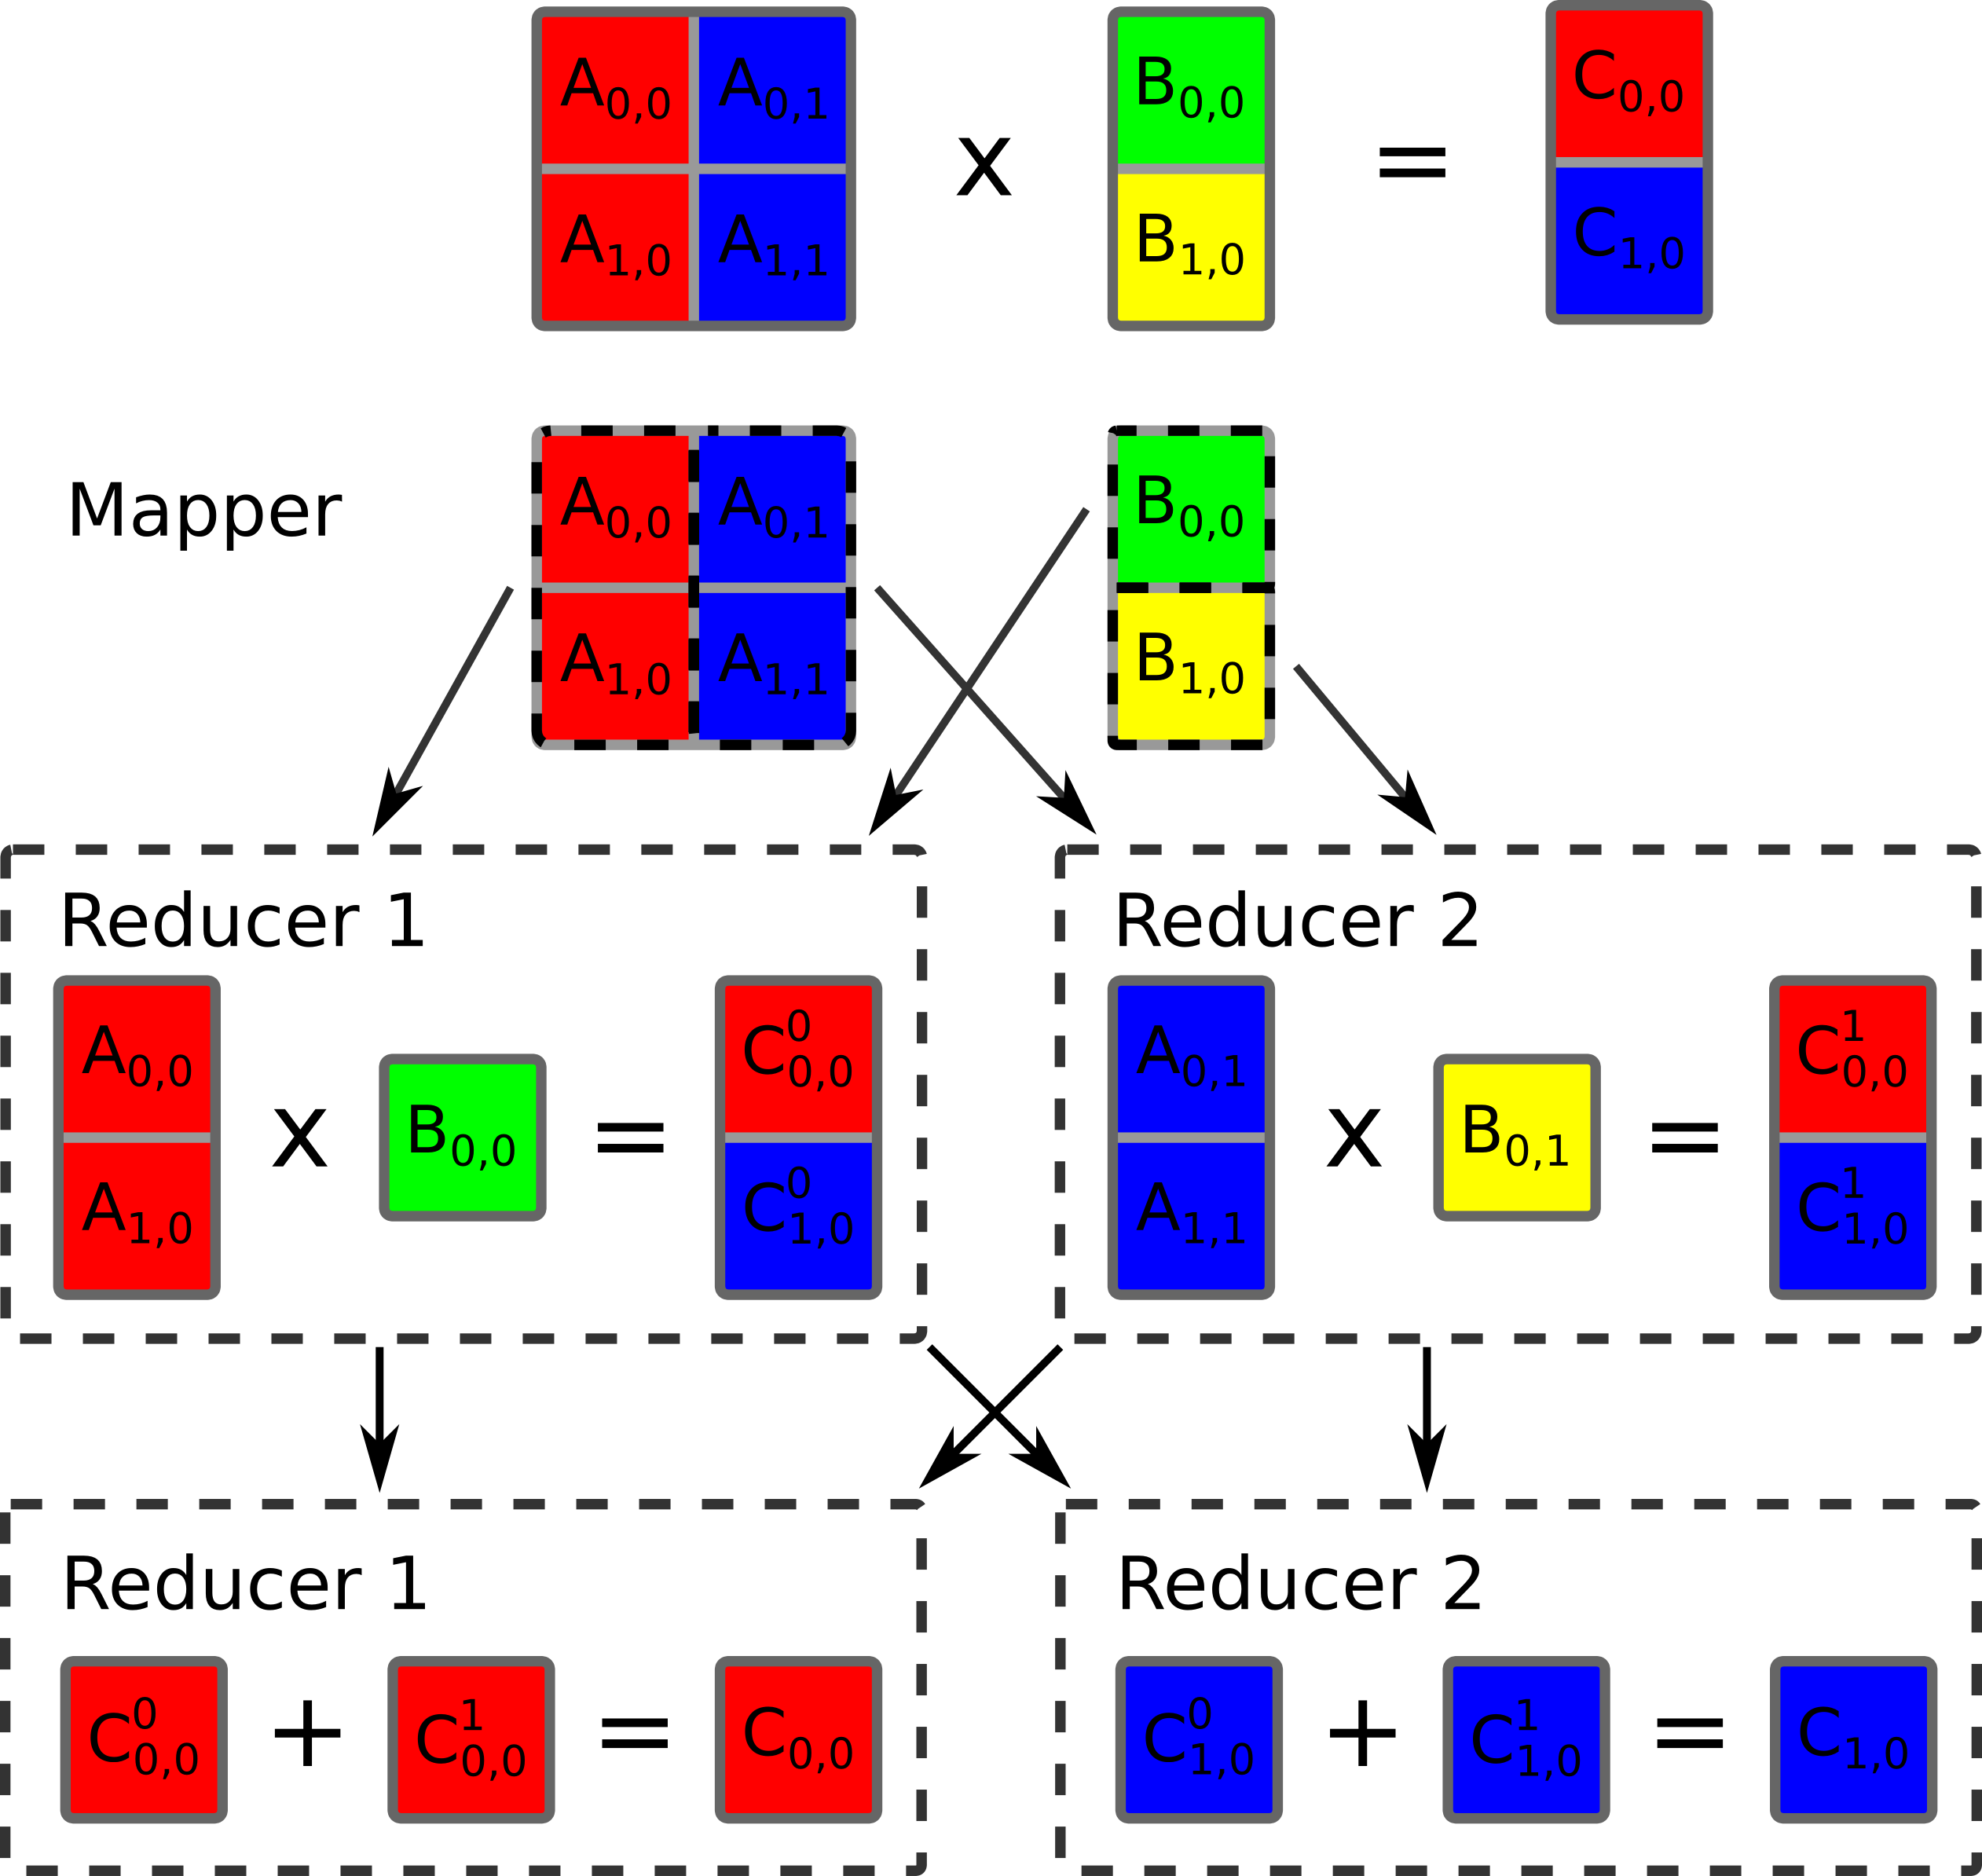
\includegraphics[width=0.8\linewidth]{images/cpmm.png}
		\caption{Cross product matrix multiplication.}
		\label{fig:CPMM}
	\end{subfigure}
	\caption{Execution strategies for matrix multiplication in MapReduce.}
	\label{fig:MMs}
\end{figure}

In contrast to RMM, CPMM calculates the outer products between $A^k$ and $B_k$ for all $k$. A mapper can group the $A^k$ and $B_k$ together so that a reducer can compute the outer products. Consequently, this method does not replicate any data. The outer product produces intermediate result matrices $C^k$ which have to be added up to produce the final result $C=\sum_{k=1}^{l} C^k$. This summation can be achieved by a subsequent reducer. The whole process is illustrated in \cref{fig:CPMM}. The methods RMM and CPMM differ in terms of network communication. The former method can be realized within a single MapReduce job whereas the latter requires two. Neither RMM nor CPMM is always superior. The optimal matrix multiplication strategy depends on the matrix size of its operands $A$ and $B$. Fortunately, Flink and Spark exhibit a little bit more flexibility in terms of higher order functions. Looking at the definition of the matrix multiplication for $C_{ij}=\sum_{k=1}^{l}A_{ik}\times B_{kj}$, it can be seen that every $A_{ik}$ has to be joined with its corresponding $B_{kj},\forall k$. This pairwise mapping can be easily achieved by using the join function. The join-key is the column index of $A$ and the row index of $B$. The joiner calculates for each matching pair $A_{ik}$ and $B_{kj}$ an intermediate result $C_{ij}^k$. Grouping the intermediate results with respect to the index pair $(i,j)$ allows us to compute the final result in a subsequent reduce step. The overall algorithm strongly resembles the CPMM. Flink supports several execution strategies for the higher-order functions. A cost-based optimizer selects the best strategies prior to execution. One possible optimization concerns the join function. The join can either be realized using a hybrid-hash join or a sort-merge join algorithm depending on the current partitioning and the input data sizes. If one input data is relatively small compared to the other input, it is usually more efficient to use the hybrid-hash join algorithm. Without loss of generality, we assume that the matrix $B$ constitutes such a small input. If we further assume that the block rows of $A$ are kept on the same worker node, then the last reduce operation can be executed locally and without any shuffling. The resulting execution plan under these assumptions is equivalent to the RMM. If the system chooses the sort-merge join algorithm instead, then the columns of $A$ will be distributed across the worker nodes. Consequently, the last reduce step causes a mandatory repartitioning. Then, the resulting execution plan is equivalent to the CPMM. Even though Gilbert has only one dataflow plan specified to implement the matrix multiplication, the Flink system can choose internally between the RMM and CPMM strategy. The strategy is selected by the optimizer which bases its decision on the data size and the partitioning, if available. %Consequently, Flink frees the programmer from this decision.
%!TEX root=paper.tex
\section{Evaluation}
\label{sec:evaluation}

In this chapter, we will investigate the scalability of Gilbert and its performance compared to well known hand-tuned ML algorithms.
We show that Gilbert is not only easily usable in terms of programming but also produces results with decent performance.

\textbf{Experimental Setup}. For our evaluation, we use a Google compute engine cluster with $8$ machines of type \code{n1-standard-16}.
Each machine is equipped with $60$ gigabytes of main memory and has $16$ virtual CPUs. 
The Spark execution engine runs on Apache Spark-2.0.0~\cite{spark}.
For the Flink execution engine, we use Apache Flink-1.1.2~\cite{flink}. 
As underlying distributed file system we use Apache Hadoop-2.7.3~\cite{hadoop:2008a}.

\subsection{Scalability}

The scalability evaluation investigates how Gilbert behaves under increasing work loads and how well it can exploit varying cluster sizes.
As we have implemented Gilbert to provide a scalable linear algebra environment, it is important that it can process data sizes exceeding the main memory of a single machine.

\textbf{Matrix Multiplication}. 
As a first benchmark, we choose the matrix multiplication $A\times B$ with $A,B \in \mathbb{R}^{n\times n}$ and $n$ being the dimensionality. 
The matrix multiplication operation is demanding, both in CPU load as well as network I/O as it requires two network shuffles. 
The matrices $A$ and $B$ are sparse matrices with uniformly distributed non-zero cells. 
They are randomly generated prior to the matrix multiplication with a sparsity of $0.001$. 
As baseline, we run the same matrix multiplication on a single machine of the cluster using Gilbert's local execution engine. 
The Flink and Spark execution engines are both started with $48$ gigabytes of main memory for their task managers and they distribute the work equally among all worker nodes. 
In the first experiment, we fixed the block sizes to $500 \times 500$ and set the number of cores to $64$. 
We then increased the dimensionality $n$ of $A$ and $B$ to observe the runtime behavior. 
The resulting execution times for the local, Flink and Spark execution engines are shown in \cref{fig:mmLoadRuntime}. 
In the second experiment, we investigate the scaling behavior of Gilbert with respect to the cluster size. 
In order to observe the communication costs, we keep the work load per core constant while increasing the number of cores. 
For this experiment we vary the number of cores from $1$ to $128$ and scale $n$ such that $n^3/\#cores$ is constant. 
We started with $n=5000$ for a single core and reached $n=25000$ on $128$ cores. 
The results of the experiment are shown in \cref{fig:mmNodesRuntime}.
\begin{figure}[htbp]
	\centering
	\begin{subfigure}{\dualpgfwidth}
		\begin{tikzpicture}
			\begin{loglogaxis}[
				xlabel={Dimensionality $n$},
				ylabel={Execution time $t$ in s},
				width=\dualpgfwidth,
				height=.78\dualpgfwidth,
				legend entries={Local, Spark, Flink},
				legend pos=north west,
				legend style={font=\scriptsize},
				font=\footnotesize
			]
			\addplot[
				color=blue,
				mark=x,
			] table[
				x=RowsA,
				y=Time,
			]
			{data/matrixMult/matrixMultLoadReference};
			\addplot[
				color=red,
				mark=o,
			] table[
				x=RowsA,
				y=Time,
			]
			{data/matrixMult/matrixMultLoadSpark};
			\addplot[
				color=teal,
				mark=triangle,
			] table[
				x=RowsA,
				y=Time,
			]
			{data/matrixMult/matrixMultLoadFlink};
			\end{loglogaxis}
		\end{tikzpicture}
		\caption{}
		\label{fig:mmLoadRuntime}
	\end{subfigure}
	\begin{subfigure}{\dualpgfwidth}
		\begin{tikzpicture}
			\begin{semilogxaxis}[
				xlabel={Number of cores},
				ylabel={Execution time $t$ in s},
				legend pos=north west,
				legend entries={Spark, Flink},
				legend style={font=\scriptsize},
				ymin=0.0,
				ymax=2000,
				width=\dualpgfwidth,
				height=.78\dualpgfwidth,
				font=\footnotesize
			]
			\addplot[
				color=red,
				mark=o,
			] table[
				x=Parallelism,
				y=Time,
			]
			{data/matrixMult/matrixMultScalabilitySpark};
			\addplot[
				color=teal,
				mark=triangle,
			] table[
				x=Parallelism,
				y=Time,
			]
			{data/matrixMult/matrixMultScalabilityFlink};
			\end{semilogxaxis}
		\end{tikzpicture}
		\caption{}
		\label{fig:mmNodesRuntime}
	\end{subfigure}
	\caption{Scalability of matrix multiplication. \subref{fig:mmLoadRuntime} Execution time of matrix multiplication depending on the data size. \subref{fig:mmNodesRuntime} Execution time of matrix multiplication depending on the cluster size with constant work load per core.}
	\label{fig:mmScalability}
\end{figure}

On a single machine, we are able to execute the matrix multiplication for dimensionalities up to $n=10000$ in a reasonable time. 
We can see that the local execution performs better for dimensionalities $n \le 2500$. 
That is expected since the matrix still fits completely in the main memory of a single machine and the distributed execution adds communication overhead and job start up latency.
For matrices with $n>2500$, Spark and Flink start to calculate the matrix multiplication faster than the local executor. 
We also see that Gilbert can handle matrix sizes which scale far beyond what a single machine can handle. 

The results depicted in \cref{fig:mmNodesRuntime} indicate for both execution engines decent scale-out behavior.
For Spark we observe an almost horizontal line for number of cores $\le 32$.
For larger number of cores, the scaling degrades which is probably caused by spilling.
The same applies to Flink.
However, we can observe that the system has to start spilling data earlier.
Thus, Flink's scale-out behavior is not as good as Spark's with respect to matrix multiplication.

\textbf{Gaussian Non-negative Matrix Factorization}. As second benchmark, we choose the Gaussian non-negative matrix factorization (GNMF) algorithm~\cite{seung:anips2001a}.
GNMF finds for a given matrix $V \in \mathbb{R}^{d\times w}$ a factorization $W \in \mathbb{R}^{d\times t}$ and $H \in \mathbb{R}^{t\times w}$ such that $V\approx W H$ holds true.
For our evaluation, we calculate one step of the GNMF algorithm.
We set $t=10$, $w=100000$ and vary the number of rows $d$ of $V$.
The matrix $V\in\mathbb{R}^{d\times 100000}$ is a sparse matrix whose sparsity is set to $0.001$.
The non-zero cells of $V$ are uniformly distributed.
As baseline, we run the GNMF on a single machine of the cluster using the local execution engine.
Like for the matrix multiplication benchmark, the task manager of Spark and Flink are started with $48$ gigabytes of memory.
In the first experiment we fix the number of cores to $64$.
We start with $d=500$ and increase the number of rows of $V$ to $150000$.
The block size of Gilbert is set to $500 \times 500$.
In order to compare the results with the optimized GNMF MapReduce implementation proposed in~\cite{liu:2010a}, we re-implemented the algorithm using  Spark and Flink.
This hand-tuned implementation, henceforth denoted as HT-GNMF (HT in the graphs), is also executed on $64$ cores.
The execution times of HT-GNMF and Gilbert's GNMF are shown in \cref{fig:nmfLoadRuntime}.
In the second experiment of the GNMF benchmark, we analyze how Gilbert scales-out when increasing the cluster size while keeping the work load for each core constant.
We vary the cluster size from $1$ core to $64$ cores and scale the number of documents $d$ accordingly.
Initially we start with $1000$ documents and, consequently, calculate the matrix factorization for $64000$ documents on $64$ cores.
The results of this experiment are shown in \cref{fig:nmfNodesRuntime}.
\begin{figure}[!h]
	\centering
	\begin{subfigure}{\dualpgfwidth}
		\begin{tikzpicture}
			\begin{loglogaxis}[
				xlabel={Number of rows of matrix $V$},
				ylabel={Execution time $t$ in s},
				width=\dualpgfwidth,
				height=.16\paperheight,
				legend pos=north west,
				legend columns=2,
				legend entries={Local, Spark, Flink, HT Spark, HT Flink},
				legend style={font=\scriptsize},
				ymax=800,
				font=\footnotesize
			]
			\addplot[
				color=blue,
				mark=x,
			] table[
				x=Rows,
				y=Time,
			]
			{data/nnmfStep/nnmfStepLoadReference};
			
			\addplot[
				color=red,
				mark=o,
			] table[
				x=Rows,
				y=Time,
			]
			{data/nnmfStep/nnmfStepLoadSpark};
			
			\addplot[
				color=teal,
				mark=triangle,
			]table[
				x=Rows,
				y=Time,
			]
			{data/nnmfStep/nnmfStepLoadFlink};
			\addplot[
				color=black,
				mark=diamond,
			]table[
				x=rowsV,
				y=time,
			]
			{data/nnmfStep/gnmfStepBenchLoadSpark};
			\addplot[
				color=magenta,
				mark=square,
			]table[
				x=rowsV,
				y=time,
			]
			{data/nnmfStep/gnmfStepBenchLoadFlink};
			\end{loglogaxis}
		\end{tikzpicture}
		\caption{}
		\label{fig:nmfLoadRuntime}
	\end{subfigure}
	\begin{subfigure}{\dualpgfwidth}
		\begin{tikzpicture}
			\begin{semilogxaxis}[
				xlabel={Number of rows of matrix $V$},
				ylabel={Speedup of HT over Gilbert},
				width=\dualpgfwidth,
				height=.16\paperheight,
				ymin=0,
				ymax=2.5,
				legend entries={Spark,Flink},
				legend pos=north west,
				legend style={font=\scriptsize},
				font=\footnotesize
			]
			\addplot[
				color=red,
				mark=o,
			] table[
				x=Rows,
				y=Speedup,
			]
			{data/nnmfStep/gnmfStepSpeedupSpark};

			\addplot[
				color=teal,
				mark=diamond,
			] table[
				x=Rows,
				y=Speedup,
			]
			{data/nnmfStep/gnmfStepSpeedupFlink};
			\end{semilogxaxis}
		\end{tikzpicture}
		\caption{}
		\label{fig:gnmfSpeedup}
	\end{subfigure}
	\begin{subfigure}{\dualpgfwidth}
		\begin{tikzpicture}
			\begin{semilogxaxis}[
				xlabel={Number of cores},
				ylabel={Execution time $t$ in s},
				xmax=101,
				ymin=0,
				ymax=60,
				legend entries={Spark, Flink},
				legend pos=north west,
				legend style={font=\scriptsize},
				width=\dualpgfwidth,
				height=.14\paperheight,
				font=\footnotesize]
			\addplot[
				color=red,
				mark=o,
			] table[
				x=Parallelism,
				y=Time,
			]
			{data/nnmfStep/nnmfStepScalabilitySpark};
			\addplot[
				color=teal,
				mark=diamond,
			] table[
				x=Parallelism,
				y=Time,
			]
			{data/nnmfStep/nnmfStepScalabilityFlink};
			\end{semilogxaxis}
		\end{tikzpicture}
		\caption{}
		\label{fig:nmfNodesRuntime}
	\end{subfigure}
	\caption{Scalability of GNMF. \subref{fig:nmfLoadRuntime} Execution time of one GNMF step depending on the data size. \subref{fig:gnmfSpeedup} Speedup of HT-GNMF over Gilbert's GNMF using Spark and Flink. \subref{fig:nmfNodesRuntime} Execution time of one GNMF step depending on the cluster size with constant work load per core.}
	\label{fig:nmfBenchmark}
\end{figure}

The local executor is applied to sizes of $d$ ranging from $500$ to $3000$ rows.
Surprisingly, the local execution is outperformed by the distributed engines.
This fact indicates that the network communication costs are not decisive.
The distributed systems can also be used for data sizes which can no longer be handled by a single machine.
Both distributed execution engines scale well and achieve almost identical results as the hand tuned implementations.
The speedup of the HT-GNMF variants compared to GNMF on Spark's and Flink's executor is shown in \cref{fig:gnmfSpeedup}.
In the case of Flink, the HT-GNMF variant runs at most $1.78$ times faster than Gilbert's GNMF implementation for large data sets.
For Spark, we can only observe a maximum speedup of $1.35$.
This result underlines Gilbert's good performance.

Furthermore, the development with Gilbert was considerably easier.
One GNMF step can be programmed in five lines of Gilbert code, whereas we needed $28$ lines of Scala code for Spark's HT-GNMF and $70$ lines of Scala code for Flink's HT-GNMF.
Not only did we have to know how to program Spark and Flink, but it also took us quite some time to verify the correct functioning of both implementations.
The verification was made significantly more difficult and time-consuming due to a programming bug we introduced.
The debugging process showed us quite plainly how tedious the development process even with systems like Spark and Flink can be.
Thus, the productivity increase gained by using a high-level declarative programming language for linear algebra must not be neglected and compensates for the slight performance loss.
\cite{alvaro:2010a} made similar observations while developing a declarative programming language for distributed systems programming.
The scale-out behavior of the Flink and Spark execution engines \cref{fig:nmfNodesRuntime} both show good results for $\#cores$ up to $64$.
The runtime on Spark with $64$ cores is only $1.26$ times slower than the runtime on a single core with the same work load per core.
For Flink we observe a slowdown of $2.38$ when running on $64$ cores.

\subsection{PageRank}

In this section, we want to investigate how well the PageRank algorithm~\cite{page:1999a} implemented in Gilbert performs compared to a specialized implementation (denoted as SP in the figures).
We expect that the Gilbert runtime adds some overhead.
Furthermore, the high-level linear algebra abstraction of Gilbert might make it difficult to exploit certain properties to speed up the processing.
We first execute PageRank directly in Gilbert, given the Gilbert code in \cref{lst:gilbertPageRank}, and then run them directly on Flink and Spark.
In contrast to Gilbert, the direct implementation requires a deep understanding of the underlying runtime system.
Furthermore, the distributed implementation is far from trivial compared to the linear algebra representation of the original problem.
\begin{listing}[htbp]
	\begin{lstlisting}[language=Matlab,
		commentstyle=\color{black},
		  stringstyle=\color{black},
		  keywordstyle=\color{black}\bfseries,
		  morekeywords={ones, fixpoint},
		  xleftmargin=.0\textwidth,
		  basicstyle=\small]
% load adjacency matrix
A = load();
maxIterations = 10;
d = sum(A, 2); % outdegree per vertex
% create the column-stochastic transition matrix
T = (diag(1 ./ d) * A)'; 
r_0 = ones(numVertices, 1) / numVertices; % initialize the ranks
e = ones(numVertices, 1) / numVertices;
% PageRank calculation
fixpoint(r_0, @(r) .85 * T * r + .15 * e, maxIterations)
	\end{lstlisting}
	\caption{Gilbert PageRank implementation.}
	\label{lst:gilbertPageRank}
\end{listing}

The specialized Spark and Flink implementation of PageRank works as follows.
The Page\-Rank vector is represented by a set of tuples $(w_i, r_i)$ with $w_i$ denoting the web site $i$ and $r_i$ being its rank.
The adjacency matrix is stored row-wise as a set of tuples $(w_i, A_i)$ with $w_i$ denoting the web site $i$ and $A_i$ being its adjacency list.
For the adjacency list $A_i$, it holds that $w_j \in A_i$ if and only if there exists a link from web site $i$ to $j$.
The next PageRank vector is calculated as follows.
The PageRank $r_i$ of web site $i$ is joined with its adjacency list $A_i$.
For each outgoing link $w_j \in A_i$ a new tuple $(w_j, 0.85r_i/\left|A_i\right|)$ with the rank of $i$ being divided by the number of outgoing links is created.
In order to incorporate the random jump behavior to any available web site, a tuple $(w_i, 0.15/|w|)$, with $|w|$ being the number of all web sites, is generated for each web site $i$.
In order to compute the next PageRank vector, all newly generated tuples are grouped according to their ID and summed up.
These steps constitute a single PageRank iteration whose data flow plan is depicted in \cref{fig:pageRankDataFlow}.
\begin{figure}[htbp]
	\centering
	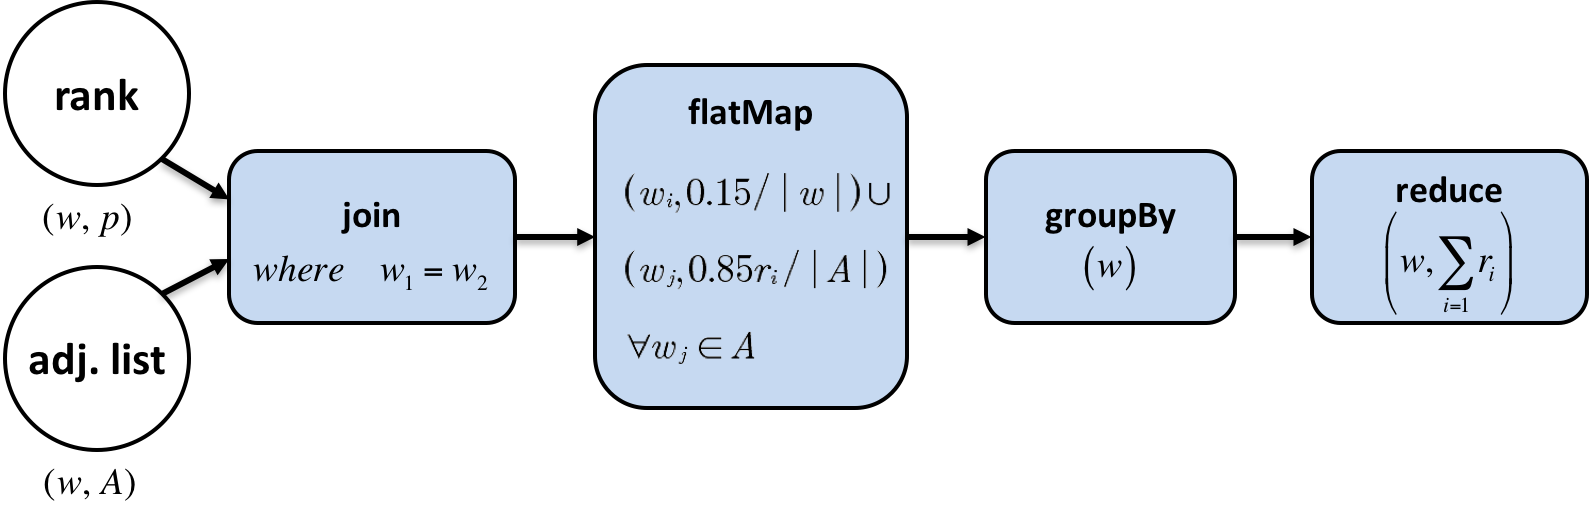
\includegraphics[width=.85\linewidth]{images/pageRankStep2.png}
	\caption{Data flow of one iteration of the PageRank algorithm for Spark and Flink.}
	\label{fig:pageRankDataFlow}
\end{figure}

\textbf{Experiment}. For comparison, $10$ steps of the PageRank algorithm for varying sizes of the adjacency matrix $A$ are calculated.
The randomly generated adjacency matrix $A$ is a sparse matrix of size $n \times n$ with a sparsity of $0.001$.
The computation is executed on $64$ cores with a block size of $500 \times 500$.
The execution times are depicted in \cref{fig:pageRankResults}.
\begin{figure}[htbp]
	\centering
	\begin{subfigure}[h]{\dualpgfwidth}
		\begin{tikzpicture}
			\begin{loglogaxis}[
				xlabel={Number of vertices $n$},
				ylabel={Execution time $t$ in s},
				xmax=250000,
				ymax=50000,
				legend pos=north west,
				legend entries={Spark, Flink, SP Flink, SP Spark},
				legend style={font=\scriptsize},
				width=\dualpgfwidth,
				height=.78\dualpgfwidth,
				font=\footnotesize
			]
			
			\addplot[blue,
				mark=x,
			] table[
				x=NumVertices,
				y=Time,
			]
			{data/pagerank/pagerankLoadSpark};

			\addplot[red,
				mark=o,
			] table[
				x=NumVertices,
				y=Time,
			]
			{data/pagerank/pagerankLoadFlink};

			\addplot[teal,
				mark=diamond,
			] table[
				x=rows,
				y=time,
			]
			{data/pagerank/pagerankBenchLoadFlink};

			\addplot[black,
				mark=triangle,
			] table[
				x=rows,
				y=time,
			]
			{data/pagerank/pagerankBenchLoadSpark};
			\end{loglogaxis}
		\end{tikzpicture}
		\caption{}
		\label{fig:pageRankResults}
	\end{subfigure}
	\begin{subfigure}[h]{\dualpgfwidth}
		\begin{tikzpicture}
			\begin{semilogxaxis}[
				xlabel={Number of vertices $n$},
				ylabel={Speedup},
				legend pos=north west,
				legend entries={SP Spark, SP Flink},
				legend style={font=\scriptsize},
				width=\dualpgfwidth,
				height=.78\dualpgfwidth,
				font=\footnotesize
			]
			
			\addplot[blue,
				mark=x,
			] table[
				x=NumVertices,
				y=Speedup,
			]
			{data/pagerank/pagerankSpeedupSpark};

			\addplot[red,
				mark=o,
			] table[
				x=NumVertices,
				y=Speedup,
			]
			{data/pagerank/pagerankSpeedupFlink};
			\end{semilogxaxis}
		\end{tikzpicture}
		\caption{}
		\label{fig:pageRankSpeedup}
	\end{subfigure}
	\caption{Comparison of Gilbert's PageRank implementation with specialized algorithms on Spark and Flink. \subref{fig:pageRankResults} Execution time of $10$ steps of the PageRank algorithm depending on the adjacency matrix's size. \subref{fig:pageRankSpeedup} Speedup of specialized algorithms with respect to Gilbert's implementations.}
	\label{fig:pageRankEvaluation}
\end{figure}

The graphs in \cref{fig:pageRankResults} show that the specialized PageRank algorithm runs faster than Gilbert's versions of PageRank.
Furthermore, the specialized algorithms show a better scalability.
The speedup of the specialized algorithms with respect to Gilbert's implementations for this experiment is shown in \cref{fig:pageRankSpeedup}.
For $n\le 50000$, the hand-tuned algorithms running on Spark and Flink show a similar speedup.
The Flink and Spark version achieve a speedup of approximately $13$ and $12$ for $n=50000$, respectively.
However, for $n = 100000$ we can observe a speedup of $76$ for the Flink specialized implementation whereas Spark reaches a speedup of $14$.
Gilbert's performance degradation with Flink is likely caused by earlier data spilling.

The performance difference between the specialized algorithm and Gilbert's version can be explained by considering the different execution plans.
As shown in \cref{fig:pageRankDataFlow}, each iteration of the specialized PageRank algorithm comprises one join, one group reduce and one flat map operation.
In contrast, each iteration of Gilbert's PageRank implementation requires two cross, two join and one reduce operation.
Thus, it can be clearly seen that Gilbert's high-level linear algebra representation adds three additional operations, with one of them being highly expensive.
Therefore, it is not surprising that the specialized PageRank algorithm performs better.
%!TEX root=paper.tex
\section{Related Work}
\label{sec:relatedWork}

{\em SystemML}~\cite{ghoting:2011a,Boehm2014,Boehm2014Hybrid,Schelter2015,Elgohary2016} aims to make machine learning algorithms run on massive datasets without burdening the user with low-level implementation details and tedious hand-tuning. 
Therefore, it provides an R-like declarative high-level language, called Declarative Machine learning Language (\emph{DML}), and compiles and optimizes the resulting programs to distributed dataflow systems. 
The linear algebra operations are translated into a directed acyclic graph of high-level operators. 
This abstract representation allows to apply several optimizations such as algebraic rewrites, choice of internal matrix representation and cost-based selection of the best execution plan. 
Afterwards these plans are translated to low-level operators and executed either in the driver memory or in parallel. 
SystemML is one of the main inspirations for Gilbert. 
While it originally only supported MapReduce as runtime, it has recently also moved to supporting more advanced dataflow systems. 
Gilbert differs from SystemML by its fixpoint operator and by leveraging the general optimizers of the underlying system (e.g., the Flink optimizer for matrix multiplication optimization, see~Section~\ref{sec:LinearAlgebraOperations}). 

{\em Samsara}~\cite{Lyubimov2016,Schelter2016} is a domain-specific language for declarative machine learning in cluster environments. 
Samsara allows its users to specify programs using a set of common matrix abstractions and linear algebraic operations, similar to R or MATLAB.
Samsara automatically compiles, optimizes and executes these programs on distributed dataflow systems. 
With Samsara mathematicians and data scientists can leverage the scalability of distributed dataflow systems via common declarative abstractions, without the need for deep knowledge about the programming and execution models of such systems. 
Samsara is part of the Apache Mahout library~\cite{mahout:2011a} and supports a variety of backends, such as Apache Spark or Apache Flink. 

{\em Ricardo}~\cite{das:2010a} uses existing technologies to implement a scalable system for statistical analysis: it executes the data shipment via Hadoop and runs the actual analytic computation by R. 
It integrates these systems via Jaql~\cite{beyer:2011a}, a declarative high-level language for data-processing on Hadoop. 
Thereby, the user can initiate the distribution, transformation and aggregation of data within Hadoop. 
Furthermore, the system supports to run R code on the worker nodes as data transformations. 
However, in this setting the user still has to explicitly specify the data-flow and the data distribution, which requires a substantial understanding of MapReduce's principles. 
{\em RHIPE}~\cite{guha:s2012a} also tries to extend R to scale to large data sets using Hadoop. 
RHIPE follows an approach called divide and recombine. 
The idea is to split the examined data up into several chunks so that they fit in the memory of a single computer. 
Next a collection of analytic methods is applied to each chunk without communicating with any other computer. 
After all chunks are evaluated, the results will be recombined in an aggregation step to create the overall analytic result. 
However, this strict execution pipeline constrains the analysis process considerably. 
A system which integrates more seamlessly into the R ecosystem is {\em pR} (parallel R)~\cite{samatova:2009a}. 
The goal is to let statisticians compute large-scale data without having to learn a new system. 
pR achieves its goal by providing a set of specialized libraries which offer parallelized versions of different algorithms using MPI.
However, MPI does not integrate well with an environment where clusters are shared and usually execute several jobs concurrently. 
Furthermore, it lacks important properties such as fault-tolerance, elasticity and reliability. 
Another related system for R is {\em rmpi}~\cite{rmpi}. 
As this is only a wrapper for the respective MPI calls, it also suffers from the aforementioned problems. 
Furthermore, there is the SparkR~\cite{Venkataraman2016} project which aims to integrate Spark's API and SQL processing capabilities into R. 

For the other popular numerical computing environment out there, namely MATLAB, also a set of parallelization tools exists. 
The most popular are the MATLAB Parallel Computing Toolbox~\cite{parallelComputingToolbox} and MATLAB Distributed Computing Server~\cite{distributedComputingServer}, which are developed by MathWorks. 
The former permits to parallelize MATLAB code on a multi-core computer and the latter scales the parallelized code up to large cluster of computing machines. 
In combination, they offer a flexible way to specify parallelism in MATLAB code. 
Besides these tools there are also other projects which try to parallelize MATLAB code. 
The most noteworthy candidates are pMatlab~\cite{bliss:ijhpca2007a} and MatlabMPI~\cite{kepner:jpdc2004a} which shall be named here for the sake of completeness. 
Unfortunately, none of these approaches is known to integrate well with the current JVM-based Hadoop ecosystem, which is becoming the main source of data in production deployments. 
Another promising research direction is the deep embedding of the APIs of dataflow systems in their host language~\cite{Alexandrov2015}, where the potential to extend this embedding and the resulting optimizations to linear algebraic operations is currently explored~\cite{Kunft2016}.
%!TEX root=main.tex
\section{Conclusion}
\label{cha:conclusion}

In the context of this thesis, we addressed the problem of managing and exploiting the ever increasing data flood.
In contrast to ever growing gathering and storage capacities, the tools to harness the collected information did not scale accordingly.
Our current analytic tools are mostly limited to data sizes which can be kept in the memory of a single machine.
Often analysts have to reduce data to make them processable, thereby missing valuable insights.
In order to analyze petabytes of data, the only viable solution is to split the work up and execute it in parallel.
However, parallel data processing is a highly complex and error-prone task.
Not only does it distract the analyst from its actual task but it also requires as skill set hardly anyone possesses.
Thus, having analytic tools, which scale to vast amounts of data while hiding the low-level implementation details, becomes an imperative.

Gilbert tackles the aforementioned problems by fusing the assets of high-level linear algebra abstractions with the power of massively parallel dataflow systems.
Gilbert is a fully functional linear algebra environment, which is programmed by the widespread MATLAB language.
Gilbert programs are executed on massively parallel dataflow systems, which allow to process data exceeding the capacity of a single computer's memory.
Gilbert only requires the user to program MATLAB code in order to use the system.
Consequently, it is usable by a wide audience of data scientists, who can easily switch to Gilbert without having to re-adapt.
These properties make Gilbert a suitable candidate for the data processing challenges of tomorrow.

Gilbert itself comprises the technology stack to parse, type and compile MATLAB code into a format which can be executed in parallel.
In order to apply high-level linear algebra optimizations, we conceived an intermediate representation for linear algebra programs.
Gilbert's optimizer exploits this representation to remove redundant transpose operations and to determine an optimal matrix multiplication order.
The optimized program is translated into an highly optimized execution plan suitable for the execution on a supported engine.
Gilbert allows the distributed execution on Spark and Stratosphere.
Additionally, it exists a local execution mode.
Gilbert was developed to be easily extensible with new execution engines.
For the local linear algebra operations the Gilbert user can choose between the Breeze and Mahout library.

Our systematical evaluation has shown that Gilbert supports all fundamental linear algebra operations, making it fully operational.
Additionally, its loop support allows to implement a wide multitude of machine learning algorithms within Gilbert.
Exemplary, we have implemented the PageRank, \kmeans and GNMF algorithm.
The code changes required to make these algorithms run in Gilbert are minimal and only concern Gilbert's loop abstraction.
Our evaluation has demonstrated the effectiveness of Gilbert's matrix multiplication reordering optimization.
Furthermore, we could observe that the matrix blocking size has strong implications on the overall performance.
The best performance is achieved with block sizes which offer a good compromise between data parallelism and data granularity.
Our benchmarks have proved that Gilbert can handle data sizes which no longer can be efficiently processed on a single computer.
Moreover, Gilbert showed a promising scale out behavior, making it a suitable candidate for large-scale data processing.

The key contributions of this thesis include the development of a scalable data analysis tool which can be programmed using the well-known MATLAB language.
That way, we made the world of distributed computing accessible for data scientists and people concerned with machine learning.
Furthermore, we researched how to implement linear algebra operations efficiently in modern parallel data flow systems, such as Spark and Stratosphere.
In line with that research was the investigation of suitable distributed data structures for the representation of matrices and vectors.
As part of the implementation of Gilbert, we also investigated how to add automatically type information to MATLAB code using a type inference mechanism.
Type inference ensures a minimally invasive approach, since the user does not have to add additional statements to his code.
Last but not least, we showed the effectiveness of a cost-based optimizer for linear algebra programs.

We also noted some limitations of Gilbert.
The proposed Hindley-Milner type inference algorithm turned out to have problems resolving polymorphic types.
As a consequence, Gilbert will incorrectly reject some well-typed programs.
However, these programs constitute only corner cases.
Even though, Gilbert can process vast amounts of data, it turned out that it cannot beat the performance of hand-tuned algorithms using Spark or Stratosphere.
Considering the overhead the linear algebra abstraction entails, this fact is not really surprising, though.
The overhead is also the reason for the higher memory foot-print, causing Spark and Stratosphere to spill faster to disk than the hand-tuned algorithms.
Consequently, the processable problem sizes are smaller.
Gilbert trades some performance off for better usability, which manifests itself in shorter and more expressive programming code.
The fact that Gilbert only supports one hard-wired partitioning scheme, namely square blocks, omits possible optimization potential.
Another limitation are the error messages of the parsing, typing and compilation phase.
It is a well known problem of the HM type inference algorithm that in case of typing errors the original error source is hard to locate.
The same holds true for issued error messages by Scala's Parser Combinators.

Interesting aspects for further research and improvements of Gilbert include the extension of the Gilbert optimizer by new optimization strategies.
The investigation of different matrix partitioning schemes and its integration into the optimizer which selects the best overall partitioning seems to be very promising.
Furthermore, a tighter coupling of Gilbert's optimizer with Stratosphere's optimizer could result in beneficial synergies.
Forwarding the inferred matrix sizes to the underlying execution system might help to improve the execution plans.
The numerical stability of Gilbert's computations is another important aspect, which has been completely left out in the context of this thesis.
However, any linear algebra environment has to guarantee numerical stability which might be influenced by Gilbert's parallel execution.
Therefore, the numerical stability of Gilbert deserves its own separate evaluation.
As stated above, the HM inference algorithm has problems with polymorphic types.
In our opinion, it is worthwhile to look into other type inference algorithms, such as the type inference system of Haskell~\cite{haskell}, to assess whether they are better suited to automatically annotate Matlab with type information.
We also strongly advise to add support for further execution engines to Gilbert.
An appropriate candidate could be the H2O~\cite{h2o} data processing engine.
Additionally, it is always beneficial to extend the set of implemented algorithms and to probe them at a large data scale.

In conclusion, we have developed Gilbert, a sparse linear algebra environment executed in massively parallel dataflow systems.
Gilbert transparently parallelizes sequential linear algebra code.
Thus, Gilbert makes it blindingly easy to develop parallel analytic tools which are capable of processing vast amounts of data.
With Gilbert at hand, we are well prepared for the looming challenges of today and tomorrow.
We believe that our system helps mankind to benefit a little bit more from the world of data.

%No \bibliography{paper} allowed here - biblatex expects it at the preamble
%Run `biber paper` to generate the bibliography
\AtNextBibliography{\footnotesize}
\printbibliography

\end{document}